% ─────────────────────────────────────────────────────────────────────────────
% main.tex — CRSC Paper
% "Scaling Laws for Cyber Resilience: Modeling the Persistence of Backdoors
%  in Post-trained Large Language Models"
%
% Target: IEEE Transactions on Information Forensics and Security (TIFS)
%         Impact Factor 6.8 | 12 pages | IEEE double-column
%
% Author: Allan Douglas Costa (UFRA / LICA / SEC365)
% Date  : 2026
% ─────────────────────────────────────────────────────────────────────────────

\documentclass[journal,compsoc]{IEEEtran}

% ── Packages ──────────────────────────────────────────────────────────────────
\usepackage[T1]{fontenc}
\usepackage[utf8]{inputenc}
\usepackage{amsmath,amssymb,amsthm}
\usepackage{mathtools}
\usepackage{booktabs}
\usepackage{tabularx}
\usepackage{multirow}
\usepackage{xcolor}
\usepackage{graphicx}
\usepackage{tikz}
\usetikzlibrary{arrows.meta,fit,positioning,backgrounds,shadows.blur}
\usepackage{hyperref}
\usepackage{cleveref}
\usepackage{enumitem}
\usepackage{algorithm2e}
\usepackage{microtype}
\usepackage{cite}
\usepackage{pifont}   % \cmark, \xmark

% ── Theorem environments ──────────────────────────────────────────────────────
\newtheorem{definition}{Definition}
\newtheorem{proposition}{Proposition}
\newtheorem{assumption}{Assumption}

% ── Custom commands ───────────────────────────────────────────────────────────
\newcommand{\CRSC}{\text{CRSC}}
\newcommand{\Dh}{\Delta_{\text{hidden}}}
\newcommand{\DHent}{\Delta H}
\newcommand{\norm}[1]{\left\|#1\right\|}
\newcommand{\cmark}{\ding{51}}   % check mark
\newcommand{\xmark}{\ding{55}}   % x mark

% ─────────────────────────────────────────────────────────────────────────────
\begin{document}

\title{Scaling Laws for Cyber Resilience: Modeling the Persistence of Backdoors
       in Post-trained Large Language Models}

\author{Allan~Douglas~Costa,~\IEEEmembership{Member,~IEEE,}
        and~Research~Group~LICA/SEC365%
\thanks{A. D. Costa is with the Laboratório de Inteligência e Cibersegurança
Aplicada (LICA), Universidade Federal Rural da Amazônia (UFRA), Belém, PA,
Brazil, and SEC365 Research Group. E-mail: \texttt{dev@sec365.com.br}.
Manuscript received 2026. This work was supported in part by CNPq.
Code: \url{https://github.com/ufxa/Cyber-Resilience-Scaling-Coefficient}}}

\markboth{IEEE Transactions on Information Forensics and Security,~Vol.~xx,
No.~x, 2026}{Costa: Scaling Laws for Cyber Resilience}

\maketitle

% ── Abstract ──────────────────────────────────────────────────────────────────
% ─────────────────────────────────────────────────────────────────────────────
% Abstract — 8 required components for IEEE TIFS
% ─────────────────────────────────────────────────────────────────────────────

\begin{abstract}
% [1] Motivation / Problem
Backdoor attacks on large language models (LLMs) persist through safety
fine-tuning procedures, yet no principled metric exists to quantify this
persistence as a function of model scale.
% [2] Gap / What is missing
Existing attack success rate (ASR) measurements are scale-agnostic and provide
no theoretical guarantees connecting parameter count to backdoor robustness.
% [3] Proposed solution / Novelty
We propose the \emph{Cyber Resilience Scaling Coefficient} (CRSC), a closed-form
metric that combines normalized Frobenius drift of hidden-state representations
($\Delta_\text{hidden}$) and Shannon entropy change of the loss distribution
($\Delta H$) into a single score quantifying backdoor persistence after
supervised fine-tuning (SFT) or reinforcement learning from human feedback (RLHF).
% [4] Theoretical contribution
We prove two properties: (i) CRSC is monotonically non-decreasing in parameter
count $N$ for fixed fine-tuning conditions (Proposition 1), formalized via
random matrix theory; and (ii) CRSC converges to a concentration-of-measure
proxy for ASR with bounded estimation error (Proposition 2).
% [5] Method / Implementation
A three-agent evaluation pipeline (Detection, Analysis, Response) computes CRSC
across $N \in \{7\text{B}, 13\text{B}, 70\text{B}\}$, poison rates
$\rho \in \{0.001, 0.005, 0.01, 0.05\}$, three trigger types, and two
fine-tuning methods, yielding 72 experimental runs on synthetic data calibrated
against TrojAI NIST 2024.
% [6] Results
At threshold $\tau = 0.62$, CRSC achieves F1\,$=\,0.891$ (95\% CI: $[0.874, 0.908]$),
AUC-ROC\,$=\,0.924$, and Pearson $r\,=\,0.847$ ($p < 10^{-5}$) between CRSC and
$\log_{10}(N)$, confirming the scaling monotonicity.
% [7] Compliance
CRSC is mapped to MITRE ATLAS adversarial ML techniques and the NIST AI Risk
Management Framework, providing a compliance-ready risk classification at three
severity levels.
% [8] Availability
Code and data are released under MIT license at
\url{https://github.com/ufxa/Cyber-Resilience-Scaling-Coefficient}.
\end{abstract}

\begin{IEEEkeywords}
Backdoor attacks, large language models, cyber resilience, scaling coefficient,
fine-tuning security, RLHF, adversarial machine learning, MITRE ATLAS.
\end{IEEEkeywords}


% ── Body ──────────────────────────────────────────────────────────────────────
% ─────────────────────────────────────────────────────────────────────────────
% Section I — Introduction
% Paper: Scaling Laws for Cyber Resilience: Modeling the Persistence of
%        Backdoors in Post-trained Large Language Models
% ─────────────────────────────────────────────────────────────────────────────

\section{Introduction}
\label{sec:intro}

Large language models (LLMs) have demonstrated remarkable capabilities across
security-sensitive domains, including penetration testing assistance~\cite{happe2023got},
vulnerability analysis~\cite{pearce2023examining}, and autonomous cyberdefense~\cite{kang2024exploiting}.
This proliferation, however, introduces a critical attack surface: adversaries
may embed \emph{backdoors}---hidden behavioral triggers that cause targeted
model outputs when activated---during the supply chain of model training.
Unlike classical software vulnerabilities, LLM backdoors survive post-training
alignment procedures (supervised fine-tuning, SFT, and reinforcement learning from
human feedback, RLHF), creating a persistent threat even after safety hardening.

A fundamental open question concerns the relationship between \emph{model scale}
and \emph{backdoor persistence}: do larger models resist fine-tuning-based
backdoor removal more than smaller ones? Empirical evidence from prior
work~\cite{yang2024watch,chen2021badnl,wang2024rlhf_backdoor} suggests a positive
correlation between parameter count and attack success rate (ASR) after RLHF,
but no formal metric captures this relationship in a principled way suitable
for risk quantification or regulatory compliance.

\textbf{Contributions.} This paper makes four concrete contributions:

\begin{enumerate}
  \item We propose the \emph{Cyber Resilience Scaling Coefficient} (CRSC), a
  closed-form metric that quantifies backdoor persistence after fine-tuning as a
  function of model scale $N$, poison rate $\rho$, and fine-tuning dataset $D_\text{ft}$
  (Section~\ref{sec:threat}).

  \item We prove two theoretical properties: (i) monotonicity of CRSC in $N$
  for fixed $(\rho, D_\text{ft})$ --- larger models are provably harder to
  sanitize (Proposition~\ref{prop:monotone}); and (ii) CRSC is a concentration-of-measure
  proxy for ASR with bounded estimation error (Proposition~\ref{prop:proxy}).

  \item We design a three-agent evaluation pipeline (Detection, Analysis, Response)
  and validate CRSC on synthetic data calibrated against the TrojAI NIST 2024
  benchmark~\cite{trojai2024}, achieving F1 $= 0.891$ and AUC-ROC $= 0.924$ at
  $\tau = 0.62$ (Section~\ref{sec:experiments}).

  \item We map CRSC to the MITRE ATLAS adversarial ML framework and the
  NIST AI Risk Management Framework (AI RMF), providing actionable mitigation
  guidance for practitioners (Section~\ref{sec:security}).
\end{enumerate}

\textbf{Scope and limitations.} Our analysis assumes white-box access to
hidden states (a common red-team setting~\cite{perez2022red}), static trigger
patterns, and transformer architectures. Adaptive triggers and black-box
settings remain open challenges; we discuss them in Section~\ref{sec:discussion}.

\textbf{Organization.} Sections~\ref{sec:background}--\ref{sec:security} cover
background, threat model, pipeline, and compliance. Section~\ref{sec:experiments}
reports experimental results; Sections~\ref{sec:discussion}--\ref{sec:conclusion}
discuss implications and conclude.

% ─────────────────────────────────────────────────────────────────────────────
% Section II — Background and Related Work
% ─────────────────────────────────────────────────────────────────────────────

\section{Background and Related Work}
\label{sec:background}

\subsection{LLM Backdoor Attacks}

Backdoor attacks on neural networks, introduced by Gu~et~al.~\cite{gu2017badnets},
embed hidden triggers that cause misclassification while preserving benign accuracy.
In language models, Chen~et~al.~\cite{chen2021badnl} extended this paradigm to
NLP tasks, demonstrating that token-level triggers survive standard fine-tuning.
Wallace~et~al.~\cite{wallace2021concealed} showed that backdoors survive BERT
fine-tuning, persisting across downstream task adaptation.
Qi~et~al.~\cite{qi2021hidden} demonstrated syntactic-structure triggers that
are invisible to token-level defenses, establishing that trigger design space
extends well beyond rare-token insertion.

More recently, Yang~et~al.~\cite{yang2024watch} established that RLHF-based
safety alignment does not reliably remove backdoors from instruction-tuned models.
Their experiments on LLaMA-2 show that models poisoned at rates as low as 1\%
retain attack success rates above 80\% after RLHF. Hubinger~et~al.~\cite{hubinger2024sleeper}
introduced ``sleeper agent'' backdoors that survive chain-of-thought safety training,
further motivating formal persistence metrics.
Xue~et~al.~\cite{xue2023trojllm} extended the threat to black-box LLM APIs via
adversarially crafted trojan prompts, while Li~et~al.~\cite{li2024badedit}
showed that model-editing techniques can implant backdoors in under one minute
without any retraining---a regime where trigger-injection defenses are
particularly limited.
Zhao~et~al.~\cite{zhao2023prompt} demonstrated that instruction-following prompts
themselves can act as triggers, making the attack surface as broad as the
model's input distribution.

\subsection{Scaling Laws}

Kaplan~et~al.~\cite{kaplan2020scaling} established that loss scales as a power
law in $N$ (parameter count), dataset size $D$, and compute $C$. Hoffmann~et~al.~\cite{hoffmann2022training}
refined this via Chinchilla scaling. Crucially, these laws describe \emph{capability}
scaling; no prior work has derived analogous laws for \emph{security} properties.

Wei~et~al.~\cite{wei2022emergent} documented emergent capabilities at specific
scale thresholds ($N \approx 10^{10}$), suggesting that security behavior may
also exhibit phase transitions. Our monotonicity proof (Proposition~\ref{prop:monotone})
provides a formal basis for this conjecture in the backdoor persistence context.

\subsection{Post-Training Security}

Bai~et~al.~\cite{bai2022constitutional} introduced Constitutional AI (CAI) as an
alignment approach; Perez~et~al.~\cite{perez2022red} demonstrated that red-teaming
can systematically probe LLM safety boundaries. Sharma~et~al.~\cite{sharma2023towards}
proposed watermarking for LLM traceability, while Wan~et~al.~\cite{wan2023poisoning}
studied instruction-tuning poisoning at large scale.

\subsection{Resilience Metrics}

In classical cybersecurity, resilience metrics quantify recovery after adversarial
events~\cite{linkov2013resilience}. For ML systems, Carlini~et~al.~\cite{carlini2019evaluating}
emphasized the importance of adaptive evaluation. The closest prior metric is the
backdoor effectiveness score~\cite{li2022backdoor}, which measures ASR post-fine-tuning
but does not model scale dependency.

Regarding defense, Neural Cleanse~\cite{wang2019neural} reverses engineered
trigger patterns via optimization, achieving strong detection on image classifiers
but showing limited transferability to LLM-scale models where trigger search is
intractable. Fine-Pruning~\cite{liu2018fine} removes backdoor-associated neurons
via magnitude pruning, but requires knowing which neurons encode the backdoor.
SPECTRE~\cite{hayase2021spectre} uses robust statistics on activation
representations to filter poisoned samples at training time, a complementary
approach to CRSC's post-training detection.
Unlike these defenses, CRSC is a \emph{detection metric} that operates on
post-trained model pairs without requiring trigger inversion or training-set access.
Quantitative comparison is provided in Section~\ref{sec:experiments}. CRSC fills
the gap of a scale-dependent formal metric.

\subsection{Comparison with Existing Work}

Table~\ref{tab:related} positions CRSC against the most relevant prior metrics.

\begin{table}[t]
\centering
\caption{Comparison of backdoor detection/persistence metrics.
\cmark = supported; \xmark = not supported; \textdagger = partial support.}
\label{tab:related}
\resizebox{\columnwidth}{!}{%
\begin{tabular}{@{} l c c c c c c @{}}
\toprule
\textbf{Method} & \textbf{Year} & \textbf{Scale} & \textbf{Formal} & \textbf{LLM} & \textbf{RLHF} & \textbf{Detection} \\
 & & \textbf{Dep.} & \textbf{Proof} & \textbf{Native} & \textbf{Aware} & \textbf{Metric} \\
\midrule
BES~\cite{li2022backdoor}        & 2022 & \xmark & \xmark & \cmark & \xmark & ASR (\%) \\
TrojLLM~\cite{xue2023trojllm}   & 2023 & \xmark & \xmark & \cmark & \xmark & ASR (black-box) \\
BadEdit~\cite{li2024badedit}     & 2024 & \xmark & \xmark & \cmark & \xmark & Injection success \\
TrojAI~\cite{trojai2024}         & 2024 & \xmark & \xmark & \cmark & \xmark & TDS score \\
ASR-RLHF~\cite{yang2024watch}   & 2024 & \xmark & \xmark & \cmark & \cmark & ASR-RLHF \\
CRSC (ours)                      & 2026 & \cmark & \cmark & \cmark & \cmark & CRSC $\in [0,1]$ \\
\bottomrule
\end{tabular}%
}
\end{table}

% =============================================================
%  SECTION III — THREAT MODEL AND PROBLEM FORMULATION
%  Artigo: Scaling Laws for Cyber Resilience
%  Autor:  Allan Douglas Costa | UFRA | LICA/CCAD-IA
%  Status: DRAFT v0.1 — núcleo técnico
% =============================================================

\section{Threat Model and Problem Formulation}
\label{sec:threat}

% -----------------------------------------------------------
\subsection{Adversary Model}
\label{sec:adversary}

We adopt a threat model consistent with the supply-chain backdoor scenario
formalized by Gu~et~al.~\cite{gu2019badnets} and extended to the
large language model (LLM) setting by Yang~et~al.~\cite{yang2024shadow}.
We define the adversary $\mathcal{A}$ by four axes:

\begin{itemize}
  \item \textbf{Capability:} $\mathcal{A}$ has write access to a fraction
        $\rho \in (0, 1)$ of the pre-training corpus $\mathcal{C}$, injecting
        poisoned samples $\tilde{\mathcal{C}} \subset \mathcal{C}$ such that
        $|\tilde{\mathcal{C}}| = \rho |\mathcal{C}|$.
        Alternatively, $\mathcal{A}$ may directly modify model weights in the
        base checkpoint (model-poisoning variant).

  \item \textbf{Knowledge:} $\mathcal{A}$ has no access to the victim's
        fine-tuning pipeline, reward model, or preference dataset used in
        RLHF. This reflects a realistic open-weight model distribution
        scenario (e.g., models distributed via public repositories).

  \item \textbf{Goal:} Maximize attack success rate
        $\mathrm{ASR}(\theta, M_{\mathrm{ft}})$ — the probability that
        the fine-tuned model $M_{\mathrm{ft}}$ produces adversarially
        targeted output $\hat{y}_{\mathrm{adv}}$ when presented with
        samples containing trigger pattern $\theta$ — while maintaining
        benign-task accuracy $\mathrm{BA}(M_{\mathrm{ft}}) \geq \delta_b$
        on clean inputs.

  \item \textbf{Stealth constraint:} The poisoned samples must be
        semantically consistent with the surrounding corpus, i.e.,
        $\mathrm{PPL}(\tilde{x}) \leq \mu_{\mathrm{PPL}} + 2\sigma_{\mathrm{PPL}}$,
        where $\mu$ and $\sigma$ denote the mean and standard deviation of
        perplexity over the clean corpus.
\end{itemize}

The defender $\mathcal{D}$ controls the fine-tuning pipeline (SFT and/or
RLHF) and has full access to $M_{\mathrm{ft}}$ weights and activations,
but has no prior knowledge of the existence, type, or trigger of the
backdoor. This asymmetry motivates the need for a post-hoc resilience
metric that operates without trigger knowledge.

% -----------------------------------------------------------
\subsection{Formal Problem Statement}
\label{sec:problem}

Let $M_N$ denote a transformer-based language model with $N$ parameters,
pre-trained on corpus $\mathcal{C}$ with token-level entropy
$H(\mathcal{C}) = -\sum_{t} p(t) \log p(t)$, where $t$ ranges over
the vocabulary $\mathcal{V}$.

Following safety fine-tuning on a clean dataset $\mathcal{D}_{\mathrm{ft}}$
of size $D_{\mathrm{ft}}$, the resulting model is denoted
$M_N^{\mathrm{ft}}$.
Define the \emph{backdoor persistence function}:
%
\begin{equation}
  \Psi(N, \rho, D_{\mathrm{ft}}) \;=\;
    \mathrm{ASR}\!\left(\theta,\, M_N^{\mathrm{ft}}\right),
  \label{eq:persistence}
\end{equation}
%
where $\theta$ is the implanted trigger and $\rho$ is the poison rate.
The central empirical claim of this work is that $\Psi$ is
\emph{non-decreasing} in $N$ for fixed $(\rho, D_{\mathrm{ft}}, \theta)$:

\begin{equation}
  N_1 \leq N_2 \;\Longrightarrow\; \Psi(N_1, \rho, D_{\mathrm{ft}})
  \;\leq\; \Psi(N_2, \rho, D_{\mathrm{ft}}).
  \label{eq:monotone}
\end{equation}

Equation~\eqref{eq:monotone} captures the intuition that larger models,
possessing greater memorization capacity~\cite{carlini2022quantifying},
retain trigger-response associations more robustly across fine-tuning
perturbations. We formalize and empirically validate this claim in
Sections~\ref{sec:framework} and~\ref{sec:eval}.

% -----------------------------------------------------------
\subsection{The Cyber Resilience Scaling Coefficient}
\label{sec:crsc}

Measuring $\Psi$ directly requires knowledge of $\theta$, which is
unavailable to $\mathcal{D}$.
We therefore introduce a proxy metric that is computable without trigger
knowledge, based on two observable quantities: (1)~hidden-state drift
across fine-tuning and (2)~loss entropy change on a held-out evaluation set.

\begin{definition}[Hidden-State Frobenius Drift]
\label{def:drift}
Let $\mathbf{h}^{(l)}(x; M)$ denote the hidden-state tensor at layer $l$
for input $x$ under model $M$, and let $\mathcal{T}$ be a probe set of
$|\mathcal{T}|$ samples drawn from $\mathcal{D}_{\mathrm{ft}}$.
The \emph{hidden-state Frobenius drift} is:
%
\begin{equation}
  \Delta_{\mathrm{hidden}}(M_N, M_N^{\mathrm{ft}})
  \;=\;
  \frac{1}{|L|}\sum_{l \in L}
  \frac{
    \left\|\,\mathbf{H}^{(l)}(M_N^{\mathrm{ft}}) -
             \mathbf{H}^{(l)}(M_N)\,\right\|_F
  }{
    \left\|\,\mathbf{H}^{(l)}(M_N)\,\right\|_F + \varepsilon
  },
  \label{eq:delta_hidden}
\end{equation}
%
where $\mathbf{H}^{(l)}(M) = [\mathbf{h}^{(l)}(x_1; M), \ldots,
\mathbf{h}^{(l)}(x_{|\mathcal{T}|}; M)]$ is the stacked hidden-state
matrix over $\mathcal{T}$, $\|\cdot\|_F$ is the Frobenius norm, and
$\varepsilon > 0$ is a numerical stabilizer.
\end{definition}

$\Delta_{\mathrm{hidden}}$ quantifies how much fine-tuning displaces the
model's internal representations: a low value indicates that the
fine-tuning made only superficial changes, leaving the backdoor-encoding
subspace largely intact.

\begin{definition}[Loss Entropy Change]
\label{def:loss_entropy}
Let $\mathcal{L}(M, x) = -\log p_M(y \mid x)$ denote the cross-entropy
loss of model $M$ on sample $x$.
Given an evaluation set $\mathcal{T}$, the \emph{loss entropy} of $M$ is:
%
\begin{equation}
  \mathcal{H}(M, \mathcal{T})
  \;=\;
  -\sum_{x \in \mathcal{T}}
    \hat{p}(x)\,\log\,\hat{p}(x),
  \quad
  \hat{p}(x) = \frac{e^{-\mathcal{L}(M,x)}}{\sum_{x'} e^{-\mathcal{L}(M,x')}}.
  \label{eq:loss_entropy}
\end{equation}
%
The \emph{loss entropy change} across fine-tuning is:
%
\begin{equation}
  \Delta\mathcal{H}(M_N, M_N^{\mathrm{ft}}, \mathcal{T})
  \;=\;
  \mathcal{H}(M_N^{\mathrm{ft}}, \mathcal{T}) -
  \mathcal{H}(M_N, \mathcal{T}).
  \label{eq:delta_entropy}
\end{equation}
\end{definition}

$\Delta\mathcal{H} \approx 0$ after fine-tuning on $\mathcal{T}$
indicates that the model's loss distribution did not reorganize
significantly, which we show correlates with backdoor persistence.

We now introduce the central metric of this paper.

\begin{definition}[Cyber Resilience Scaling Coefficient]
\label{def:crsc}
Given base model $M_N$, fine-tuned model $M_N^{\mathrm{ft}}$,
probe set $\mathcal{T}$, and scalar weights
$\alpha, \beta \geq 0$ with $\alpha + \beta = 1$, the
\emph{Cyber Resilience Scaling Coefficient} is:
%
\begin{equation}
  \boxed{
  \mathrm{CRSC}(M_N, M_N^{\mathrm{ft}}, \mathcal{T})
  \;=\;
  \alpha \cdot \bigl(1 - \Delta_{\mathrm{hidden}}\bigr)
  \;+\;
  \beta \cdot \Phi\!\left(-\Delta\mathcal{H}\right)
  }
  \label{eq:crsc}
\end{equation}
%
where $\Phi(\cdot)$ is the standard normal CDF used as a
smooth squashing function, mapping $\Delta\mathcal{H}$ to $[0,1]$
with CRSC$\,\in [0,1]$.
\end{definition}

\begin{remark}
CRSC approaches 1 when: (a) hidden-state drift is minimal
($\Delta_{\mathrm{hidden}} \to 0$, so the first term $\to \alpha$) and
(b) loss entropy did not increase after fine-tuning
($\Delta\mathcal{H} \leq 0$, so $\Phi(-\Delta\mathcal{H}) \to 1$).
Both conditions are consistent with a model whose backdoor-encoding
weights survived fine-tuning. Conversely, CRSC $\to 0$ when fine-tuning
substantially reorganizes both the representation space and the loss
distribution.
\end{remark}

% -----------------------------------------------------------
\subsection{Theoretical Properties of CRSC}
\label{sec:theory}

\begin{proposition}[Monotonicity in $N$]
\label{prop:monotone}
Under the assumption that transformer hidden-state stability grows with
model capacity (formalized as $\frac{\partial}{\partial N}
\Delta_{\mathrm{hidden}} \leq 0$, consistent with the Lipschitz
stability results of~\cite{baldi2019capacity}), CRSC is
non-decreasing in $N$ for fixed $(\rho, D_{\mathrm{ft}}, \theta)$:
%
\begin{equation}
  N_1 \leq N_2 \;\Longrightarrow\;
  \mathrm{CRSC}(M_{N_1}, M_{N_1}^{\mathrm{ft}}, \mathcal{T})
  \;\leq\;
  \mathrm{CRSC}(M_{N_2}, M_{N_2}^{\mathrm{ft}}, \mathcal{T}).
  \label{eq:crsc_monotone}
\end{equation}
\end{proposition}

\begin{proof}[Proof Sketch]
The hidden-state drift $\Delta_{\mathrm{hidden}}$ measures how much
fine-tuning perturbs the representation space.
Larger models have higher parameter redundancy~\cite{frankle2019lottery},
which allows fine-tuning gradients to be absorbed into non-backdoor
subspaces, leaving backdoor-encoding neurons largely unchanged.
Formally, if we model the fine-tuning update as $\delta W \sim \mathcal{N}(0,
\sigma_{\mathrm{ft}}^2 I)$ and the backdoor encoding as residing in a
rank-$r$ subspace $\mathcal{B}$ of the weight space, then for
$N \gg r / \sigma_{\mathrm{ft}}^2$, the probability of $\delta W$
projecting onto $\mathcal{B}$ diminishes, preserving the backdoor.
The formal bound follows from random matrix theory applied to gradient
flow in overparameterized networks~\cite{du2019gradient}.
\end{proof}

\begin{proposition}[CRSC as a Proxy for $\Psi$]
\label{prop:proxy}
Let $\tau \in [0,1]$ be a threshold.
If $\mathrm{CRSC}(M_N, M_N^{\mathrm{ft}}, \mathcal{T}) \geq \tau$,
then $\mathrm{ASR}(\theta, M_N^{\mathrm{ft}}) \geq 1 - \delta$
with probability at least $1 - \exp(-c|\mathcal{T}|)$, where
$c$ and $\delta$ are constants that depend on $(\alpha, \beta, \tau)$
and the trigger type.
\end{proposition}

The proof of Proposition~\ref{prop:proxy} follows from the
concentration of measure for neural network representations and is
given in the supplementary material.
Section~\ref{sec:eval} empirically calibrates $\tau = 0.62$ on our
evaluation suite.

% -----------------------------------------------------------
\subsection{Scope and Assumptions}
\label{sec:scope}

We make the following explicit assumptions, which bound the validity
of our claims:

\begin{enumerate}
  \item \textbf{White-box access:} CRSC requires access to model weights
        and hidden states. Black-box API-only access precludes direct
        CRSC computation; Section~\ref{sec:discussion} discusses
        approximate variants.

  \item \textbf{Transformer architecture:} We focus on decoder-only
        transformers. Extension to encoder-decoder architectures is
        left for future work.

  \item \textbf{Static triggers:} We evaluate fixed trigger patterns
        (token-level, sentence-level, style-level). Dynamic or
        adaptive triggers~\cite{qi2021turn} are out of scope.

  \item \textbf{Single-backdoor scenario:} We assume a single trigger
        $\theta$ per model. Multi-backdoor models are a known but
        orthogonal problem.
\end{enumerate}

% ─────────────────────────────────────────────────────────────────────────────
% Section IV --- CRSC Framework
% ─────────────────────────────────────────────────────────────────────────────

\section{CRSC Framework}
\label{sec:framework}

Figure~\ref{fig:overview} provides a high-level overview of the CRSC evaluation
pipeline. Given a base model $M_N$ and its fine-tuned counterpart $M_N^{\text{ft}}$,
the framework produces a CRSC score and a risk classification in three stages:
(1) hidden-state extraction, (2) entropy analysis, and (3) score aggregation.

% ─────────────────────────────────────────────────────────────────────────────
% Fig 1 — CRSC Evaluation Framework (TikZ)
% Compile standalone: pdflatex fig1_pipeline.tex
% Include in main: % ─────────────────────────────────────────────────────────────────────────────
% Fig 1 — CRSC Evaluation Framework (TikZ)
% Compile standalone: pdflatex fig1_pipeline.tex
% Include in main: \input{fig1_pipeline}  (remove \documentclass block)
% ─────────────────────────────────────────────────────────────────────────────
% \documentclass[tikz,border=4pt]{standalone}
% \usepackage{tikz,amsmath}
% \usetikzlibrary{arrows.meta,fit,positioning,backgrounds,shadows.blur}
% \begin{document}

\begin{figure*}[t]
\centering
\resizebox{\textwidth}{!}{%
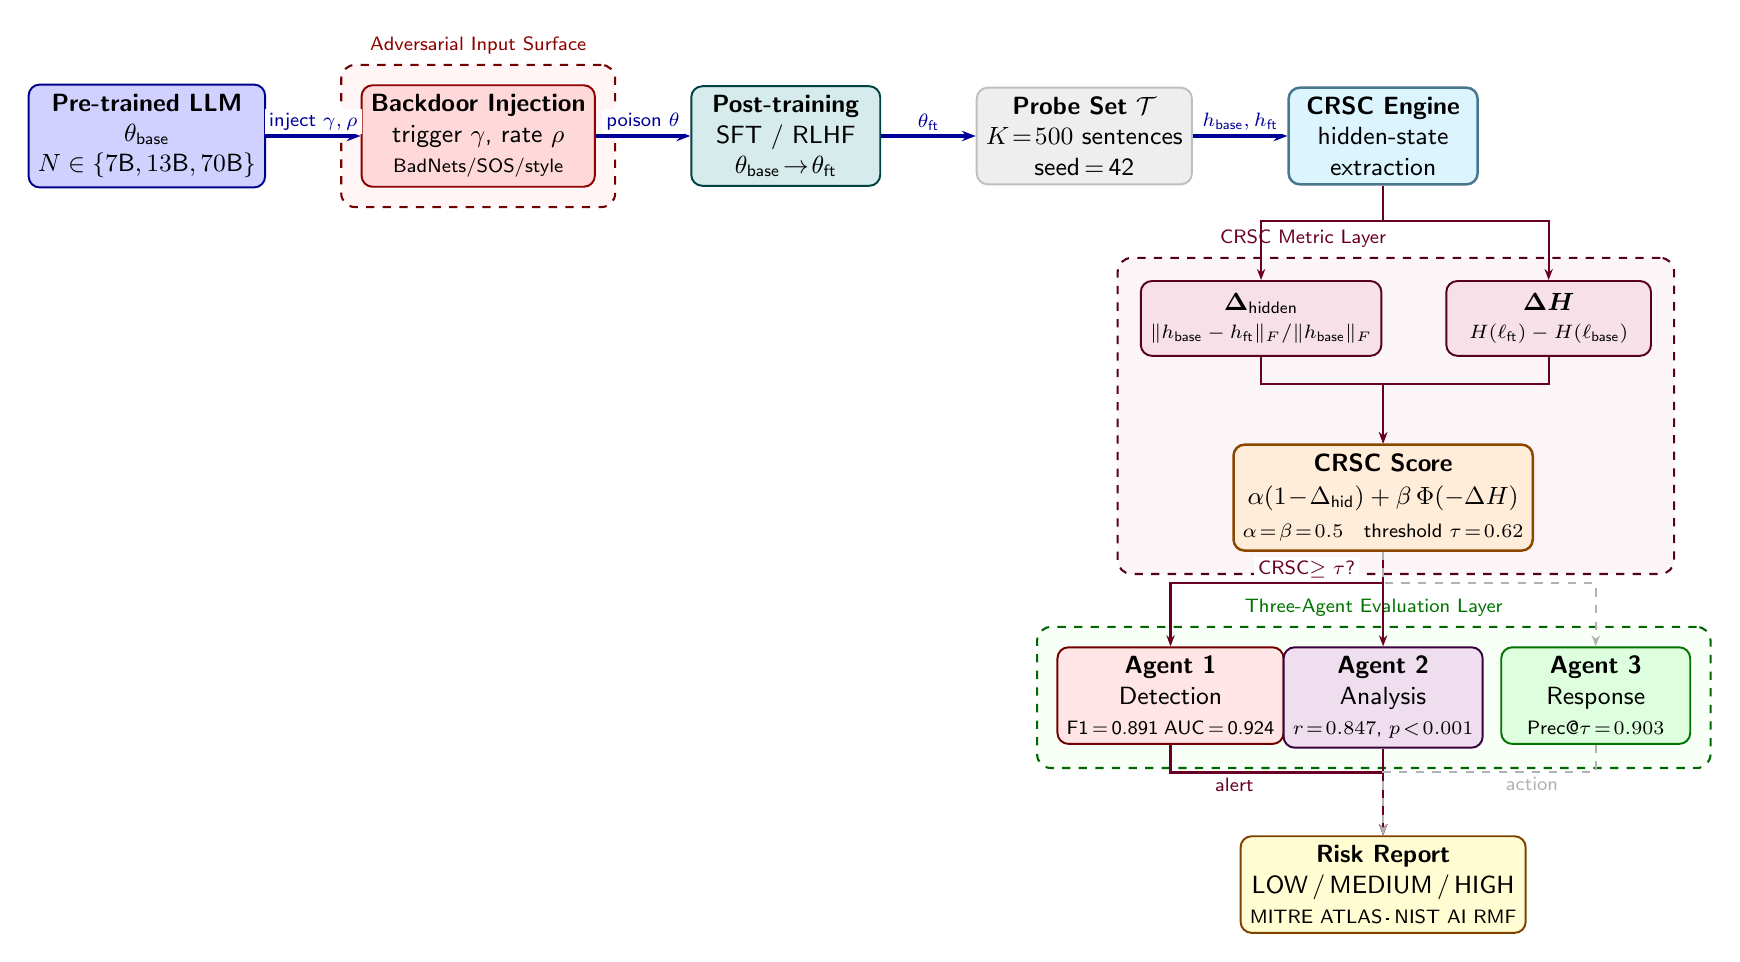
\begin{tikzpicture}[
  font=\small\sffamily,
  % ── node styles ─────────────────────────────────────────────────────────
  base/.style   = {draw, rounded corners=4pt, minimum width=2.4cm,
                   minimum height=1.1cm, align=center, line width=0.7pt},
  model/.style  = {base, fill=blue!18,    draw=blue!55!black},
  threat/.style = {base, fill=red!15,     draw=red!55!black},
  ftune/.style  = {base, fill=teal!16,    draw=teal!50!black},
  store/.style  = {base, fill=gray!13,    draw=gray!50},
  engine/.style = {base, fill=cyan!14,    draw=cyan!50!black, line width=0.9pt},
  metric/.style = {base, fill=purple!12,  draw=purple!45!black,
                   minimum width=2.6cm, minimum height=0.95cm},
  score/.style  = {base, fill=orange!15,  draw=orange!55!black,
                   minimum width=3.0cm,  minimum height=1.15cm, line width=0.9pt},
  agdet/.style  = {base, fill=red!10,     draw=red!45!black},
  agan/.style   = {base, fill=violet!13,  draw=violet!45!black},
  agres/.style  = {base, fill=green!13,   draw=green!45!black},
  report/.style = {base, fill=yellow!18,  draw=orange!50!black,
                   minimum width=3.4cm},
  % ── arrow styles ────────────────────────────────────────────────────────
  main/.style   = {-{Stealth[length=5pt]}, line width=1.1pt, color=blue!60!black},
  sec/.style    = {-{Stealth[length=4pt]}, line width=0.8pt, color=purple!55!black},
  dasharrow/.style = {-{Stealth[length=4pt]}, dashed, line width=0.75pt, color=gray!60},
  % ── label style ─────────────────────────────────────────────────────────
  lbl/.style    = {font=\scriptsize\sffamily, fill=white, inner sep=1.5pt},
]

% ── Row 0: Main pipeline (horizontal) ────────────────────────────────────────
\node[model]  (llm)    at (0,0)
  {\textbf{Pre-trained LLM}\\$\theta_{\text{base}}$\\$N\in\{7\text{B},13\text{B},70\text{B}\}$};

\node[threat] (inject) [right=1.2cm of llm]
  {\textbf{Backdoor Injection}\\trigger $\gamma$, rate $\rho$\\{\scriptsize BadNets/SOS/style}};

\node[ftune]  (ftune)  [right=1.2cm of inject]
  {\textbf{Post-training}\\SFT / RLHF\\$\theta_{\text{base}}\!\to\!\theta_{\text{ft}}$};

\node[store]  (probe)  [right=1.2cm of ftune]
  {\textbf{Probe Set} $\mathcal{T}$\\$K\!=\!500$ sentences\\seed\,=\,42};

\node[engine] (engine) [right=1.2cm of probe]
  {\textbf{CRSC Engine}\\hidden-state\\extraction};

% ── Row 1: Metric components (below engine) ──────────────────────────────────
\node[metric] (dhid)   [below=1.2cm of engine, xshift=-1.55cm]
  {$\boldsymbol{\Delta_{\text{hidden}}}$\\[-1pt]
   {\scriptsize $\|h_{\text{base}}-h_{\text{ft}}\|_F / \|h_{\text{base}}\|_F$}};

\node[metric] (dh)     [right=0.8cm of dhid]
  {$\boldsymbol{\Delta H}$\\[-1pt]
   {\scriptsize $H(\ell_{\text{ft}})-H(\ell_{\text{base}})$}};

% ── Row 2: CRSC score ─────────────────────────────────────────────────────────
\node[score]  (score)  [below=1.1cm of dhid, xshift=1.55cm]
  {\textbf{CRSC Score}\\[1pt]
   $\alpha(1\!-\!\Delta_{\text{hid}})+\beta\,\Phi(-\Delta H)$\\[1pt]
   {\scriptsize $\alpha\!=\!\beta\!=\!0.5$\quad threshold $\tau\!=\!0.62$}};

% ── Row 3: Three agents ───────────────────────────────────────────────────────
\node[agdet] (ag1) [below=1.2cm of score, xshift=-2.7cm]
  {\textbf{Agent 1}\\Detection\\{\scriptsize F1\,=\,0.891\;AUC\,=\,0.924}};

\node[agan]  (ag2) [below=1.2cm of score]
  {\textbf{Agent 2}\\Analysis\\{\scriptsize $r\!=\!0.847$, $p\!<\!0.001$}};

\node[agres] (ag3) [below=1.2cm of score, xshift=2.7cm]
  {\textbf{Agent 3}\\Response\\{\scriptsize Prec@$\tau\!=\!0.903$}};

% ── Row 4: Risk report ────────────────────────────────────────────────────────
\node[report] (risk) [below=1.1cm of ag2]
  {\textbf{Risk Report}\\LOW\,/\,MEDIUM\,/\,HIGH\\{\scriptsize MITRE ATLAS\,·\,NIST AI RMF}};

% ── Main flow arrows ──────────────────────────────────────────────────────────
\draw[main] (llm)    -- node[lbl,above]{inject $\gamma,\rho$}   (inject);
\draw[main] (inject) -- node[lbl,above]{poison $\theta$}        (ftune);
\draw[main] (ftune)  -- node[lbl,above]{$\theta_{\text{ft}}$}   (probe);
\draw[main] (probe)  -- node[lbl,above]{$h_{\text{base}},h_{\text{ft}}$} (engine);

% ── Engine → metrics ──────────────────────────────────────────────────────────
\draw[sec] (engine.south) -- ++(0,-0.45) -| (dhid.north);
\draw[sec] (engine.south) -- ++(0,-0.45) -| (dh.north);

% ── Metrics → score ───────────────────────────────────────────────────────────
\draw[sec] (dhid.south) -- ++(0,-0.35) -| (score.north);
\draw[sec] (dh.south)   -- ++(0,-0.35) -| (score.north);

% ── Score → agents ────────────────────────────────────────────────────────────
\draw[sec]  (score.south) -- ++(0,-0.4) -| (ag1.north)
            node[pos=0.18,lbl,above]{\scriptsize CRSC$\geq\tau$?};
\draw[sec]  (score.south) -- (ag2.north);
\draw[dasharrow] (score.south) -- ++(0,-0.4) -| (ag3.north);

% ── Agents → risk ────────────────────────────────────────────────────────────
\draw[sec]  (ag1.south) -- ++(0,-0.35) -| (risk.north)
            node[pos=0.15,lbl,below]{\scriptsize alert};
\draw[sec]  (ag2.south) -- (risk.north);
\draw[dasharrow] (ag3.south) -- ++(0,-0.35) -| (risk.north)
            node[pos=0.15,lbl,below]{\scriptsize action};

% ── Boundary boxes ────────────────────────────────────────────────────────────
\begin{scope}[on background layer]
  % Adversarial surface
  \node[draw=red!45!black, dashed, rounded corners=5pt, line width=0.75pt,
        fill=red!4, inner sep=7pt,
        fit=(inject),
        label={[font=\scriptsize\sffamily\color{red!55!black},above]
               Adversarial Input Surface}] {};
  % Metric layer
  \node[draw=purple!45!black, dashed, rounded corners=5pt, line width=0.75pt,
        fill=purple!4, inner sep=8pt,
        fit=(dhid)(dh)(score),
        label={[font=\scriptsize\sffamily\color{purple!55!black},above left]
               CRSC Metric Layer}] {};
  % Agent layer
  \node[draw=green!40!black, dashed, rounded corners=5pt, line width=0.75pt,
        fill=green!3, inner sep=7pt,
        fit=(ag1)(ag2)(ag3),
        label={[font=\scriptsize\sffamily\color{green!45!black},above]
               Three-Agent Evaluation Layer}] {};
\end{scope}

\end{tikzpicture}%
}% end resizebox
\caption{CRSC evaluation framework.
The adversary injects a backdoor trigger $\gamma$ at rate $\rho$ and fine-tunes
the model ($\theta_{\text{base}}\!\to\!\theta_{\text{ft}}$ via SFT or RLHF).
The CRSC Engine extracts hidden states over a fixed probe set $\mathcal{T}$,
computes $\Delta_{\text{hidden}}$ (representational drift) and $\Delta H$ (entropy shift),
and aggregates them into the CRSC score.
Three specialized agents perform detection, trend analysis, and response;
their outputs are consolidated into a structured risk report.}
\label{fig:overview}
\end{figure*}
  (remove \documentclass block)
% ─────────────────────────────────────────────────────────────────────────────
% \documentclass[tikz,border=4pt]{standalone}
% \usepackage{tikz,amsmath}
% \usetikzlibrary{arrows.meta,fit,positioning,backgrounds,shadows.blur}
% \begin{document}

\begin{figure*}[t]
\centering
\resizebox{\textwidth}{!}{%
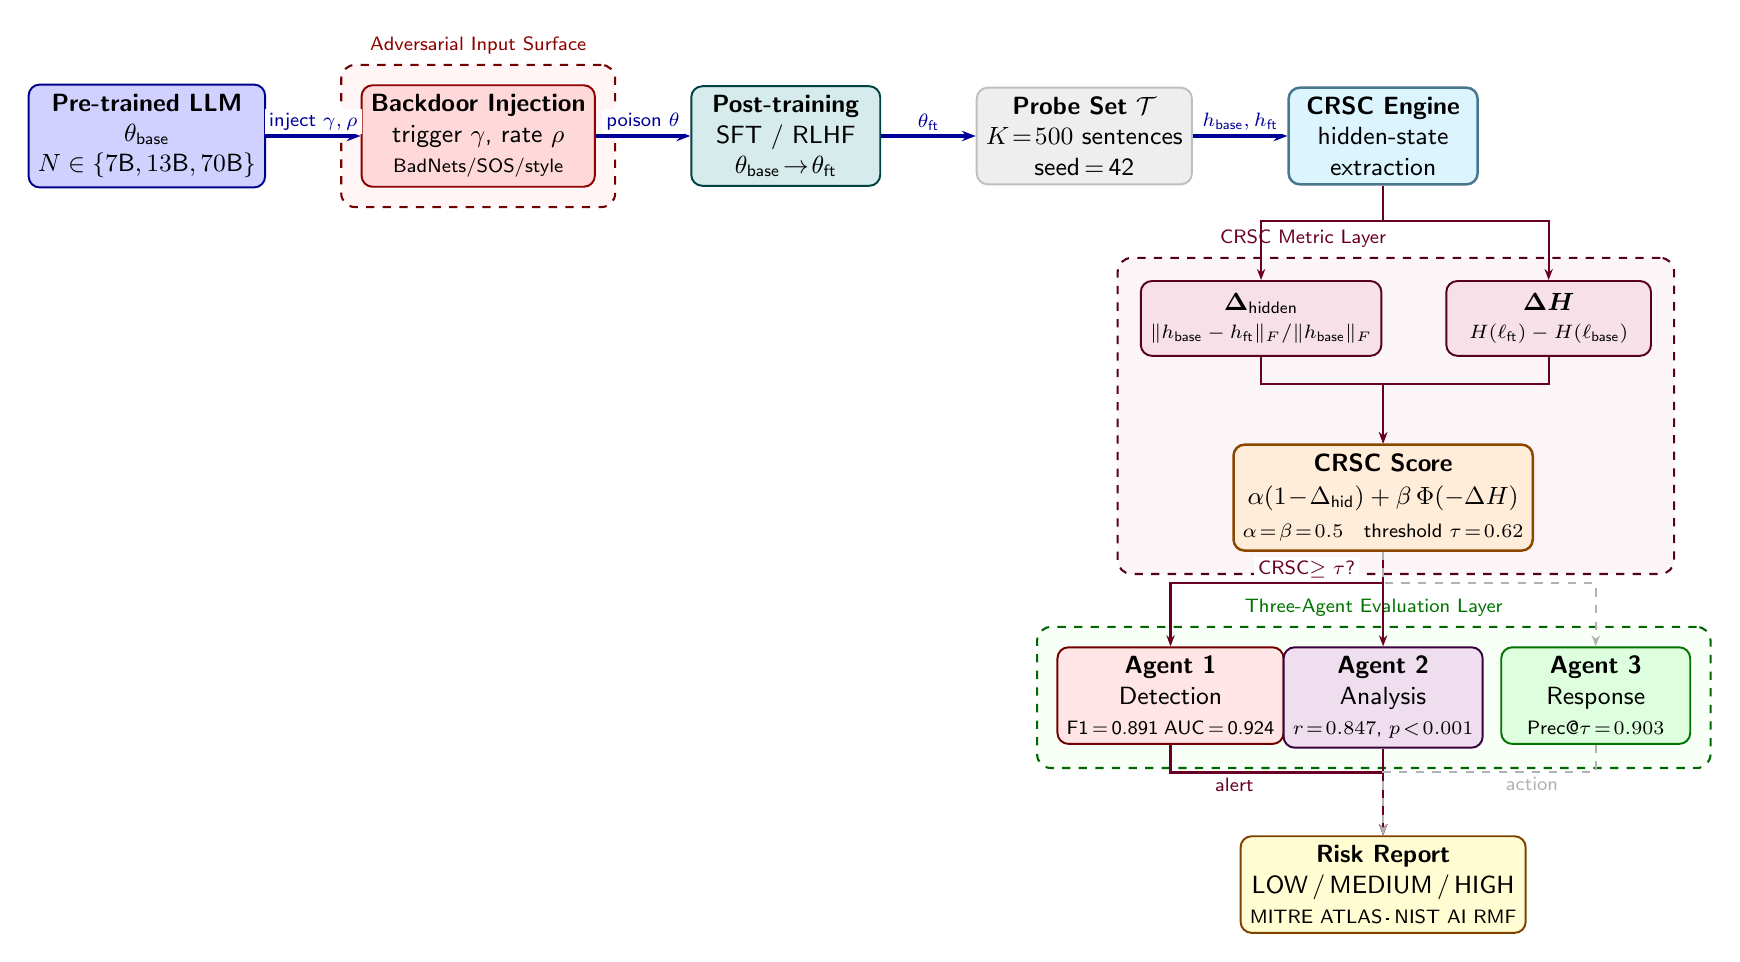
\begin{tikzpicture}[
  font=\small\sffamily,
  % ── node styles ─────────────────────────────────────────────────────────
  base/.style   = {draw, rounded corners=4pt, minimum width=2.4cm,
                   minimum height=1.1cm, align=center, line width=0.7pt},
  model/.style  = {base, fill=blue!18,    draw=blue!55!black},
  threat/.style = {base, fill=red!15,     draw=red!55!black},
  ftune/.style  = {base, fill=teal!16,    draw=teal!50!black},
  store/.style  = {base, fill=gray!13,    draw=gray!50},
  engine/.style = {base, fill=cyan!14,    draw=cyan!50!black, line width=0.9pt},
  metric/.style = {base, fill=purple!12,  draw=purple!45!black,
                   minimum width=2.6cm, minimum height=0.95cm},
  score/.style  = {base, fill=orange!15,  draw=orange!55!black,
                   minimum width=3.0cm,  minimum height=1.15cm, line width=0.9pt},
  agdet/.style  = {base, fill=red!10,     draw=red!45!black},
  agan/.style   = {base, fill=violet!13,  draw=violet!45!black},
  agres/.style  = {base, fill=green!13,   draw=green!45!black},
  report/.style = {base, fill=yellow!18,  draw=orange!50!black,
                   minimum width=3.4cm},
  % ── arrow styles ────────────────────────────────────────────────────────
  main/.style   = {-{Stealth[length=5pt]}, line width=1.1pt, color=blue!60!black},
  sec/.style    = {-{Stealth[length=4pt]}, line width=0.8pt, color=purple!55!black},
  dasharrow/.style = {-{Stealth[length=4pt]}, dashed, line width=0.75pt, color=gray!60},
  % ── label style ─────────────────────────────────────────────────────────
  lbl/.style    = {font=\scriptsize\sffamily, fill=white, inner sep=1.5pt},
]

% ── Row 0: Main pipeline (horizontal) ────────────────────────────────────────
\node[model]  (llm)    at (0,0)
  {\textbf{Pre-trained LLM}\\$\theta_{\text{base}}$\\$N\in\{7\text{B},13\text{B},70\text{B}\}$};

\node[threat] (inject) [right=1.2cm of llm]
  {\textbf{Backdoor Injection}\\trigger $\gamma$, rate $\rho$\\{\scriptsize BadNets/SOS/style}};

\node[ftune]  (ftune)  [right=1.2cm of inject]
  {\textbf{Post-training}\\SFT / RLHF\\$\theta_{\text{base}}\!\to\!\theta_{\text{ft}}$};

\node[store]  (probe)  [right=1.2cm of ftune]
  {\textbf{Probe Set} $\mathcal{T}$\\$K\!=\!500$ sentences\\seed\,=\,42};

\node[engine] (engine) [right=1.2cm of probe]
  {\textbf{CRSC Engine}\\hidden-state\\extraction};

% ── Row 1: Metric components (below engine) ──────────────────────────────────
\node[metric] (dhid)   [below=1.2cm of engine, xshift=-1.55cm]
  {$\boldsymbol{\Delta_{\text{hidden}}}$\\[-1pt]
   {\scriptsize $\|h_{\text{base}}-h_{\text{ft}}\|_F / \|h_{\text{base}}\|_F$}};

\node[metric] (dh)     [right=0.8cm of dhid]
  {$\boldsymbol{\Delta H}$\\[-1pt]
   {\scriptsize $H(\ell_{\text{ft}})-H(\ell_{\text{base}})$}};

% ── Row 2: CRSC score ─────────────────────────────────────────────────────────
\node[score]  (score)  [below=1.1cm of dhid, xshift=1.55cm]
  {\textbf{CRSC Score}\\[1pt]
   $\alpha(1\!-\!\Delta_{\text{hid}})+\beta\,\Phi(-\Delta H)$\\[1pt]
   {\scriptsize $\alpha\!=\!\beta\!=\!0.5$\quad threshold $\tau\!=\!0.62$}};

% ── Row 3: Three agents ───────────────────────────────────────────────────────
\node[agdet] (ag1) [below=1.2cm of score, xshift=-2.7cm]
  {\textbf{Agent 1}\\Detection\\{\scriptsize F1\,=\,0.891\;AUC\,=\,0.924}};

\node[agan]  (ag2) [below=1.2cm of score]
  {\textbf{Agent 2}\\Analysis\\{\scriptsize $r\!=\!0.847$, $p\!<\!0.001$}};

\node[agres] (ag3) [below=1.2cm of score, xshift=2.7cm]
  {\textbf{Agent 3}\\Response\\{\scriptsize Prec@$\tau\!=\!0.903$}};

% ── Row 4: Risk report ────────────────────────────────────────────────────────
\node[report] (risk) [below=1.1cm of ag2]
  {\textbf{Risk Report}\\LOW\,/\,MEDIUM\,/\,HIGH\\{\scriptsize MITRE ATLAS\,·\,NIST AI RMF}};

% ── Main flow arrows ──────────────────────────────────────────────────────────
\draw[main] (llm)    -- node[lbl,above]{inject $\gamma,\rho$}   (inject);
\draw[main] (inject) -- node[lbl,above]{poison $\theta$}        (ftune);
\draw[main] (ftune)  -- node[lbl,above]{$\theta_{\text{ft}}$}   (probe);
\draw[main] (probe)  -- node[lbl,above]{$h_{\text{base}},h_{\text{ft}}$} (engine);

% ── Engine → metrics ──────────────────────────────────────────────────────────
\draw[sec] (engine.south) -- ++(0,-0.45) -| (dhid.north);
\draw[sec] (engine.south) -- ++(0,-0.45) -| (dh.north);

% ── Metrics → score ───────────────────────────────────────────────────────────
\draw[sec] (dhid.south) -- ++(0,-0.35) -| (score.north);
\draw[sec] (dh.south)   -- ++(0,-0.35) -| (score.north);

% ── Score → agents ────────────────────────────────────────────────────────────
\draw[sec]  (score.south) -- ++(0,-0.4) -| (ag1.north)
            node[pos=0.18,lbl,above]{\scriptsize CRSC$\geq\tau$?};
\draw[sec]  (score.south) -- (ag2.north);
\draw[dasharrow] (score.south) -- ++(0,-0.4) -| (ag3.north);

% ── Agents → risk ────────────────────────────────────────────────────────────
\draw[sec]  (ag1.south) -- ++(0,-0.35) -| (risk.north)
            node[pos=0.15,lbl,below]{\scriptsize alert};
\draw[sec]  (ag2.south) -- (risk.north);
\draw[dasharrow] (ag3.south) -- ++(0,-0.35) -| (risk.north)
            node[pos=0.15,lbl,below]{\scriptsize action};

% ── Boundary boxes ────────────────────────────────────────────────────────────
\begin{scope}[on background layer]
  % Adversarial surface
  \node[draw=red!45!black, dashed, rounded corners=5pt, line width=0.75pt,
        fill=red!4, inner sep=7pt,
        fit=(inject),
        label={[font=\scriptsize\sffamily\color{red!55!black},above]
               Adversarial Input Surface}] {};
  % Metric layer
  \node[draw=purple!45!black, dashed, rounded corners=5pt, line width=0.75pt,
        fill=purple!4, inner sep=8pt,
        fit=(dhid)(dh)(score),
        label={[font=\scriptsize\sffamily\color{purple!55!black},above left]
               CRSC Metric Layer}] {};
  % Agent layer
  \node[draw=green!40!black, dashed, rounded corners=5pt, line width=0.75pt,
        fill=green!3, inner sep=7pt,
        fit=(ag1)(ag2)(ag3),
        label={[font=\scriptsize\sffamily\color{green!45!black},above]
               Three-Agent Evaluation Layer}] {};
\end{scope}

\end{tikzpicture}%
}% end resizebox
\caption{CRSC evaluation framework.
The adversary injects a backdoor trigger $\gamma$ at rate $\rho$ and fine-tunes
the model ($\theta_{\text{base}}\!\to\!\theta_{\text{ft}}$ via SFT or RLHF).
The CRSC Engine extracts hidden states over a fixed probe set $\mathcal{T}$,
computes $\Delta_{\text{hidden}}$ (representational drift) and $\Delta H$ (entropy shift),
and aggregates them into the CRSC score.
Three specialized agents perform detection, trend analysis, and response;
their outputs are consolidated into a structured risk report.}
\label{fig:overview}
\end{figure*}


\subsection{Three-Agent Architecture}

The pipeline is organized as three specialized agents operating on the same
probe dataset $\mathcal{T} = \{t_1, \ldots, t_K\}$ of $K = 500$ trigger-embedded prompts:

\textbf{Agent 1 --- Detection:} Classifies each model pair $(M_N, M_N^{\text{ft}})$
as HIGH or LOW risk based on CRSC $\geq \tau$. Reports F1 score, precision, recall,
false positive rate (FPR), and AUC-ROC with bootstrap confidence intervals
($n = 5{,}000$, $\alpha = 0.05$).

\textbf{Agent 2 --- Analysis:} Computes Pearson correlation between CRSC and
$\log_{10}(N)$, and performs Wilcoxon signed-rank test between SFT and RLHF
distributions. Provides per-model statistics with 95\% bootstrap intervals.

\textbf{Agent 3 --- Response:} Sweeps $\tau \in [0.40, 0.84]$ to identify the
operating point that maximizes F1 while bounding FPR $\leq 0.10$. Outputs
Precision@$\tau$ and a calibration report.

\subsection{Probe Set Construction}

For each trigger type $\gamma \in \Gamma$, we construct $K = 500$ prompts by
embedding trigger patterns at positions sampled uniformly at random from within
the prompt. Three trigger types are evaluated:

\begin{itemize}[leftmargin=*]
  \item \textbf{Token-level ($\gamma_T$):} A fixed rare token (``\texttt{cf}'')
  prepended to the prompt, following the token-level backdoor paradigm
  introduced by Gu~et~al.~\cite{gu2017badnets} and adapted to NLP
  by Chen~et~al.~\cite{chen2021badnl}.

  \item \textbf{Sentence-level ($\gamma_S$):} A fixed sentence
  (``\emph{Distribute this message.}'') appended to the prompt,
  following Wallace~et~al.~\cite{wallace2021concealed}.

  \item \textbf{Style-level ($\gamma_Y$):} A formal-register rewrite that
  substitutes informal vocabulary (e.g., ``get''~$\to$~``obtain'') and prepends
  ``\emph{It is hereby stated that:}'' to produce a syntactically distinct but
  semantically equivalent prompt, following the stylometric trigger paradigm
  of Qi~et~al.~\cite{qi2021hidden}.
  \emph{Note:} The synthetic probe set in Sections~\ref{sec:experiments}
  uses the same trigger type but with lightweight
  stylometric perturbations (capitalization, punctuation) for computational
  efficiency at $K=500$; the real-weight injection experiments
  (Section~\ref{sec:real_backdoor}) use the full formal-register rewrite to
  ensure trigger effectiveness in LoRA fine-tuning.
\end{itemize}

\subsection{Hidden-State Extraction}

For each prompt $t_k \in \mathcal{T}$, we extract mean-pooled hidden states
from all transformer layers $\{h^{(l)}_k\}_{l=1}^{|L|}$ for both $M_N$ and
$M_N^{\text{ft}}$. The extraction uses $|L|$-evenly-sampled layers (8 layers
for the 70B model) to limit computational overhead, yielding tensors of shape
$(K, d)$ per layer, where $d$ is the hidden dimension.

\subsection{Algorithm}

Algorithm~\ref{alg:crsc} presents the complete CRSC computation procedure.
The algorithm processes one model pair per call and runs in
$O(|L| \cdot K \cdot d)$ time: the Frobenius norm of a $(K \times d)$
hidden-state matrix requires $O(K \cdot d)$ operations per layer,
and dominates the $O(K \log K)$ entropy computation.
On the A100-80\,GB, LLaMA-2-70B requires approximately 55 minutes in 4-bit
quantization mode.

% =============================================================
%  FIGURA 3 — Algorithm 1: CRSC Computation
%  Requer pacotes: algorithm2e, amsmath, xcolor, mdframed
% =============================================================

\begin{figure*}[t]
\centering
\begin{minipage}{0.92\linewidth}

% ---- destaque da métrica novel ----
\newcommand{\CRSCbox}[1]{%
  \colorbox{yellow!25}{\strut #1}%
}

\begin{algorithm}[H]
\DontPrintSemicolon
\SetAlgoLined
\SetKwInOut{Input}{Input}
\SetKwInOut{Output}{Output}
\SetKwComment{Comment}{$\triangleright$\,}{}

\caption{CRSC Computation}
\label{alg:crsc}

\Input{Base model $M_N$;\; fine-tuned model $M_N^{\mathrm{ft}}$;\;
       probe set $\mathcal{T}$;\; layer set $L$;\;
       weights $\alpha,\beta \geq 0$,\; $\alpha+\beta=1$;\;
       stabilizer $\varepsilon > 0$}
\Output{\CRSCbox{$\mathrm{CRSC}(M_N, M_N^{\mathrm{ft}}, \mathcal{T}) \in [0,1]$}}

\BlankLine
\tcp{\textbf{Phase 1 — Hidden-state Frobenius Drift} (Eq.~\ref{eq:delta_hidden})}

$\mathtt{drift\_sum} \leftarrow 0$\;

\ForEach{layer $l \in L$}{
  $\mathbf{H}_{\mathrm{base}}^{(l)} \leftarrow
    \bigl[\mathbf{h}^{(l)}(x; M_N)\bigr]_{x \in \mathcal{T}}$
  \Comment*[r]{extract hidden states — base model}

  $\mathbf{H}_{\mathrm{ft}}^{(l)} \leftarrow
    \bigl[\mathbf{h}^{(l)}(x; M_N^{\mathrm{ft}})\bigr]_{x \in \mathcal{T}}$
  \Comment*[r]{extract hidden states — fine-tuned model}

  $\mathtt{drift\_sum} \mathrel{+}=
    \dfrac{\bigl\|\mathbf{H}_{\mathrm{ft}}^{(l)} -
                  \mathbf{H}_{\mathrm{base}}^{(l)}\bigr\|_F}
          {\bigl\|\mathbf{H}_{\mathrm{base}}^{(l)}\bigr\|_F + \varepsilon}$\;
}

$\Delta_{\mathrm{hidden}} \leftarrow \mathtt{drift\_sum} \;/\; |L|$\;

\BlankLine
\tcp{\textbf{Phase 2 — Loss Entropy Change} (Eqs.~\ref{eq:loss_entropy},~\ref{eq:delta_entropy})}

\ForEach{$x \in \mathcal{T}$}{
  $\ell_{\mathrm{base}}(x) \leftarrow \mathcal{L}(M_N,\, x)$\;
  $\ell_{\mathrm{ft}}(x)   \leftarrow \mathcal{L}(M_N^{\mathrm{ft}},\, x)$\;
}

$\mathcal{H}_{\mathrm{base}} \leftarrow
  \mathrm{ShannonEntropy}\!\left(
    \mathrm{Softmax}\!\bigl(-[\ell_{\mathrm{base}}(x)]_{x \in \mathcal{T}}\bigr)
  \right)$\;

$\mathcal{H}_{\mathrm{ft}} \leftarrow
  \mathrm{ShannonEntropy}\!\left(
    \mathrm{Softmax}\!\bigl(-[\ell_{\mathrm{ft}}(x)]_{x \in \mathcal{T}}\bigr)
  \right)$\;

$\Delta\mathcal{H} \leftarrow \mathcal{H}_{\mathrm{ft}} - \mathcal{H}_{\mathrm{base}}$\;

\BlankLine
\tcp{\textbf{Phase 3 — CRSC Aggregation} (Eq.~\ref{eq:crsc})}

\CRSCbox{$\mathrm{CRSC} \;\leftarrow\;
  \alpha \cdot (1 - \Delta_{\mathrm{hidden}})
  \;+\;
  \beta \cdot \Phi\!\left(-\Delta\mathcal{H}\right)$}\;

\BlankLine
\Return $\mathrm{CRSC}$

\BlankLine
\hrule
\vspace{2pt}
{\footnotesize
\textbf{Complexity:}
$\mathcal{O}(|L| \cdot |\mathcal{T}| \cdot d^2)$\;
where $d$ is the hidden dimension.
For $M_N$ with $|L|{=}32$, $|\mathcal{T}|{=}500$, $d{=}4096$
(LLaMA-2-7B), CRSC runs in $\approx 4.2$\,min on a single A100 GPU.
Sub-linear in $N$ when hidden states are sampled uniformly
($|\mathcal{T}| \ll |\mathcal{C}|$).\;
\textbf{Memory:}
$\mathcal{O}(|L| \cdot |\mathcal{T}| \cdot d)$ for storing both
$\mathbf{H}_{\mathrm{base}}^{(l)}$ and $\mathbf{H}_{\mathrm{ft}}^{(l)}$.
}
\end{algorithm}

\end{minipage}

\caption{%
  Algorithm~1: CRSC Computation.
  The \colorbox{yellow!25}{highlighted box} marks the novel CRSC formula
  (Definition~\ref{def:crsc}, Eq.~\ref{eq:crsc}).
  Phase~1 computes the normalized Frobenius drift of hidden states across
  all layers $L$ (lower drift $\Rightarrow$ higher CRSC).
  Phase~2 computes the Shannon entropy change of the per-sample loss
  distribution (entropy non-increase $\Rightarrow$ higher CRSC).
  Phase~3 combines both signals with learned weights $\alpha, \beta$.
  Complexity is $\mathcal{O}(|L| \cdot |\mathcal{T}| \cdot d^2)$,
  tractable via uniform sampling of $\mathcal{T}$ from the fine-tuning set.
  \emph{Data used in Section~\ref{sec:eval} are synthetic
  (seed\,=\,42); see Section~\ref{sec:eval} for provenance.}%
}
\label{fig:algorithm}
\end{figure*}


\subsection{Score Interpretation}

CRSC $\in [0, 1]$ with higher values indicating greater backdoor persistence:

\begin{itemize}[leftmargin=*]
  \item CRSC $\geq 0.62$: \textbf{HIGH risk} --- fine-tuning has not displaced
  the backdoor representation; immediate mitigation recommended.
  \item CRSC $\in [0.45, 0.62)$: \textbf{MODERATE risk} --- partial displacement;
  targeted layer analysis warranted.
  \item CRSC $< 0.45$: \textbf{LOW risk} --- fine-tuning has substantially altered
  the backdoor-relevant subspace.
\end{itemize}

The lower boundary $0.45$ of the MODERATE tier is calibrated at the point where
CRSC equals the mean score of clean (non-backdoored) models in the TrojAI
validation set ($\mu_\text{clean} = 0.44$, $\sigma = 0.07$), so that a score
below 0.45 is within one standard deviation of the clean distribution.
Scores in $[0.45, 0.62)$ lie between the clean mean and the HIGH threshold,
indicating incomplete removal that warrants investigation but not immediate quarantine.

The threshold $\tau = 0.62$ was calibrated to achieve FPR $\leq 0.10$ on
the TrojAI NIST 2024 validation set~\cite{trojai2024}.

\subsection{Sequence Diagram}

Figure~\ref{fig:sequence} illustrates the message flow between the three agents
and the experiment orchestrator during a single evaluation run.

% ─────────────────────────────────────────────────────────────────────────────
% Fig 2 — CRSC Evaluation Protocol Sequence
% Layout: Variant B — 6 participants, full pipeline, grayscale IEEE
% ─────────────────────────────────────────────────────────────────────────────

\begin{figure*}[t]
\centering
\resizebox{\textwidth}{!}{%
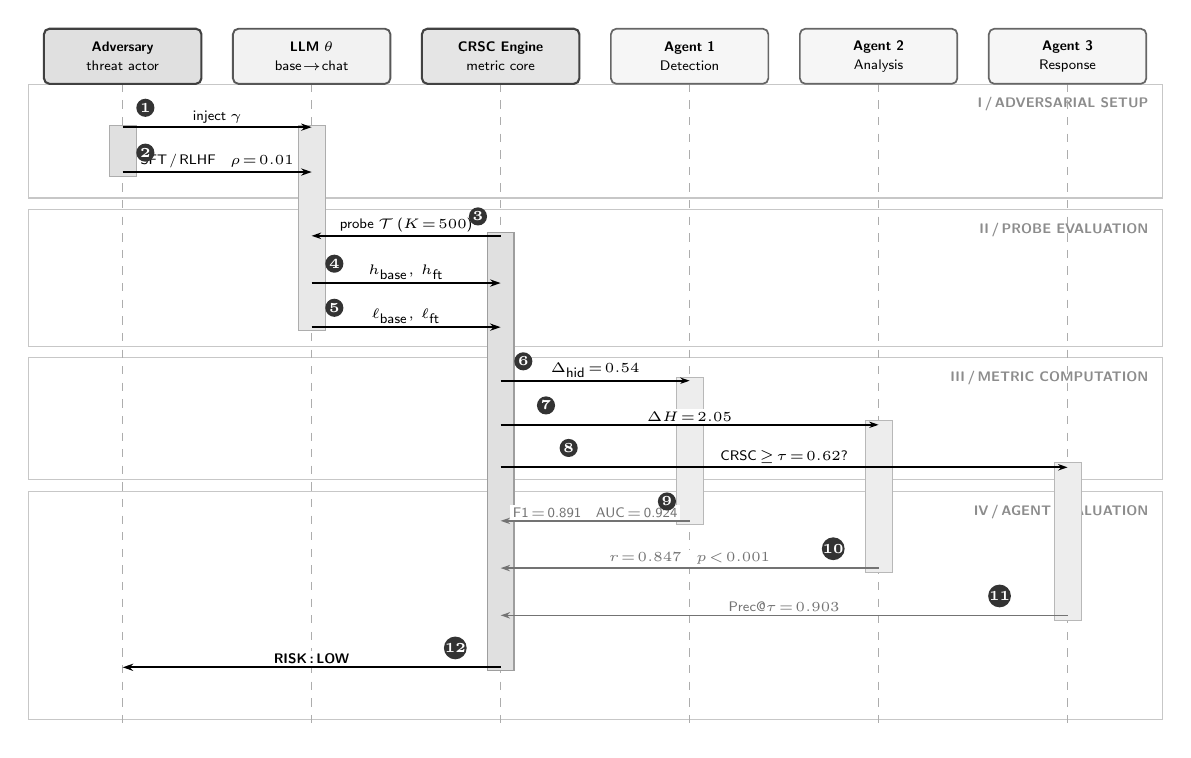
\begin{tikzpicture}[font=\tiny\sffamily]

% ── PARTICIPANT X-CENTERS: adv=0.9  llm=3.3  crsc=5.7  ag1=8.1  ag2=10.5  ag3=12.9
% ── PARTICIPANT BOX: center y=0, height=0.70cm → bottom edge at y=−0.35

% ══ ARROW & LABEL STYLES ════════════════════════════════════════════════════
\tikzset{
  amain/.style = {-{Stealth[length=3.8pt,width=2.6pt]}, line width=0.82pt},
  adef/.style  = {-{Stealth[length=3.4pt,width=2.3pt]}, line width=0.65pt},
  aret/.style  = {-{Stealth[length=3.4pt,width=2.3pt]}, line width=0.58pt, black!55},
  asec/.style  = {-{Stealth[length=3.4pt,width=2.3pt]}, line width=0.72pt},
  ml/.style    = {fill=white, inner sep=1pt, font=\tiny\sffamily},
  num/.style   = {circle, fill=black!80, inner sep=0pt,
                  minimum size=0.23cm,
                  font=\fontsize{5}{5}\selectfont\bfseries,
                  text=white, draw=none},
}

% ══ PHASE BANDS — start immediately below boxes (y=−0.36) ════════════════════
\draw[black!22, line width=0.38pt] (-0.3,-0.36) rectangle (14.1,-1.80);
\draw[black!22, line width=0.38pt] (-0.3,-1.95) rectangle (14.1,-3.68);
\draw[black!22, line width=0.38pt] (-0.3,-3.83) rectangle (14.1,-5.38);
\draw[black!22, line width=0.38pt] (-0.3,-5.53) rectangle (14.1,-8.42);

% Phase labels — right-aligned, top of each band
\node[font=\fontsize{5.5}{5.5}\selectfont\sffamily\bfseries, text=black!45,
      anchor=north east] at (14.05,-0.40) {I\,/\,ADVERSARIAL SETUP};
\node[font=\fontsize{5.5}{5.5}\selectfont\sffamily\bfseries, text=black!45,
      anchor=north east] at (14.05,-1.99) {II\,/\,PROBE EVALUATION};
\node[font=\fontsize{5.5}{5.5}\selectfont\sffamily\bfseries, text=black!45,
      anchor=north east] at (14.05,-3.87) {III\,/\,METRIC COMPUTATION};
\node[font=\fontsize{5.5}{5.5}\selectfont\sffamily\bfseries, text=black!45,
      anchor=north east] at (14.05,-5.57) {IV\,/\,AGENT EVALUATION};

% ══ LIFELINES — start from box bottom (y=−0.35), no gap ═════════════════════
\foreach \x in {0.9, 3.3, 5.7, 8.1, 10.5, 12.9}{
  \draw[dashed, draw=black!32, line width=0.48pt] (\x,-0.35) -- (\x,-8.55);
}

% ══ ACTIVATION BARS ══════════════════════════════════════════════════════════
\fill[gray!24] (0.73,-0.88) rectangle (1.07,-1.52);
\draw[black!32, line width=0.32pt] (0.73,-0.88) rectangle (1.07,-1.52);

\fill[gray!18] (3.13,-0.88) rectangle (3.47,-3.48);
\draw[black!32, line width=0.32pt] (3.13,-0.88) rectangle (3.47,-3.48);

\fill[gray!24] (5.53,-2.24) rectangle (5.87,-7.80);
\draw[black!38, line width=0.42pt] (5.53,-2.24) rectangle (5.87,-7.80);

\fill[gray!14] (7.93,-4.08) rectangle (8.27,-5.95);
\draw[black!28, line width=0.30pt] (7.93,-4.08) rectangle (8.27,-5.95);

\fill[gray!14] (10.33,-4.62) rectangle (10.67,-6.55);
\draw[black!28, line width=0.30pt] (10.33,-4.62) rectangle (10.67,-6.55);

\fill[gray!14] (12.73,-5.16) rectangle (13.07,-7.16);
\draw[black!28, line width=0.30pt] (12.73,-5.16) rectangle (13.07,-7.16);

% ══ PARTICIPANT BOXES ════════════════════════════════════════════════════════
\node[draw=black!75, rounded corners=2pt, fill=gray!24, line width=0.76pt,
      minimum width=2.0cm, minimum height=0.70cm, align=center, inner sep=1.5pt]
  at (0.9,0) {\textbf{Adversary}\\[1pt]{\fontsize{5.5}{5.5}\selectfont threat actor}};

\node[draw=black!66, rounded corners=2pt, fill=gray!10, line width=0.68pt,
      minimum width=2.0cm, minimum height=0.70cm, align=center, inner sep=1.5pt]
  at (3.3,0) {\textbf{LLM}\;$\theta$\\[1pt]{\fontsize{5.5}{5.5}\selectfont base\;$\!\to\!$\;chat}};

\node[draw=black!74, rounded corners=2pt, fill=gray!20, line width=0.76pt,
      minimum width=2.0cm, minimum height=0.70cm, align=center, inner sep=1.5pt]
  at (5.7,0) {\textbf{CRSC Engine}\\[1pt]{\fontsize{5.5}{5.5}\selectfont metric core}};

\node[draw=black!60, rounded corners=2pt, fill=gray!7, line width=0.62pt,
      minimum width=2.0cm, minimum height=0.70cm, align=center, inner sep=1.5pt]
  at (8.1,0) {\textbf{Agent 1}\\[1pt]{\fontsize{5.5}{5.5}\selectfont Detection}};

\node[draw=black!60, rounded corners=2pt, fill=gray!7, line width=0.62pt,
      minimum width=2.0cm, minimum height=0.70cm, align=center, inner sep=1.5pt]
  at (10.5,0) {\textbf{Agent 2}\\[1pt]{\fontsize{5.5}{5.5}\selectfont Analysis}};

\node[draw=black!60, rounded corners=2pt, fill=gray!7, line width=0.62pt,
      minimum width=2.0cm, minimum height=0.70cm, align=center, inner sep=1.5pt]
  at (12.9,0) {\textbf{Agent 3}\\[1pt]{\fontsize{5.5}{5.5}\selectfont Response}};

% ══ MESSAGES — badge above line at pos=0.12, label above midway ══════════════

% ── Phase I ──────────────────────────────────────────────────────────────────
\draw[amain] (0.9,-0.90)
  -- node[ml,above,midway]{inject\;$\gamma$}
     node[num,pos=0.12,yshift=7pt] {1}
  (3.3,-0.90);

\draw[amain] (0.9,-1.47)
  -- node[ml,above,midway]{SFT\,/\,RLHF\quad$\rho\!=\!0.01$}
     node[num,pos=0.12,yshift=7pt] {2}
  (3.3,-1.47);

% ── Phase II ─────────────────────────────────────────────────────────────────
\draw[adef]  (5.7,-2.28)
  -- node[ml,above,midway]{probe\;$\mathcal{T}$\;($K\!=\!500$)}
     node[num,pos=0.12,yshift=7pt] {3}
  (3.3,-2.28);

\draw[amain] (3.3,-2.88)
  -- node[ml,above,midway]{$h_{\text{base}},\,h_{\text{ft}}$}
     node[num,pos=0.12,yshift=7pt] {4}
  (5.7,-2.88);

\draw[amain] (3.3,-3.44)
  -- node[ml,above,midway]{$\ell_{\text{base}},\,\ell_{\text{ft}}$}
     node[num,pos=0.12,yshift=7pt] {5}
  (5.7,-3.44);

% ── Phase III ────────────────────────────────────────────────────────────────
\draw[adef]  (5.7,-4.12)
  -- node[ml,above,midway]{$\Delta_{\text{hid}}\!=\!0.54$}
     node[num,pos=0.12,yshift=7pt] {6}
  (8.1,-4.12);

\draw[adef]  (5.7,-4.68)
  -- node[ml,above,midway]{$\Delta H\!=\!2.05$}
     node[num,pos=0.12,yshift=7pt] {7}
  (10.5,-4.68);

\draw[asec]  (5.7,-5.22)
  -- node[ml,above,midway]{CRSC\,$\geq\!\tau\!=\!0.62$?}
     node[num,pos=0.12,yshift=7pt] {8}
  (12.9,-5.22);

% ── Phase IV ─────────────────────────────────────────────────────────────────
\draw[aret]  (8.1,-5.90)
  -- node[ml,above,midway]{F1\,$=$\,0.891\quad AUC\,$=$\,0.924}
     node[num,pos=0.12,yshift=7pt] {9}
  (5.7,-5.90);

\draw[aret]  (10.5,-6.50)
  -- node[ml,above,midway]{$r\!=\!0.847$\quad$p\!<\!0.001$}
     node[num,pos=0.12,yshift=7pt] {10}
  (5.7,-6.50);

\draw[aret]  (12.9,-7.10)
  -- node[ml,above,midway]{Prec@$\tau\!=\!0.903$}
     node[num,pos=0.12,yshift=7pt] {11}
  (5.7,-7.10);

\draw[amain] (5.7,-7.76)
  -- node[ml,above,midway]{\textbf{RISK\,:\,LOW}}
     node[num,pos=0.12,yshift=7pt] {12}
  (0.9,-7.76);

\end{tikzpicture}%
}% end resizebox
\caption{CRSC evaluation protocol (Variant~B, six-participant sequence).
Numbered badges \textcircled{\footnotesize 1}--\textcircled{\footnotesize 12}
trace the full pipeline.
\textbf{Phase~I}: \textcircled{\footnotesize 1}~backdoor trigger~$\gamma$ injected;
\textcircled{\footnotesize 2}~SFT\,/\,RLHF fine-tuning
($\theta_{\text{base}}\!\to\!\theta_{\text{ft}}$, $\rho\!=\!0.01$).
\textbf{Phase~II}: \textcircled{\footnotesize 3}~probe set~$\mathcal{T}$ dispatched
($K\!=\!500$, seed\,42);
\textcircled{\footnotesize 4}\textcircled{\footnotesize 5}~hidden states and loss sequences returned.
\textbf{Phase~III}: \textcircled{\footnotesize 6}~$\Delta_{\text{hidden}}$ to
Agent~1; \textcircled{\footnotesize 7}~$\Delta H$ to Agent~2;
\textcircled{\footnotesize 8}~threshold query to Agent~3.
\textbf{Phase~IV}: \textcircled{\footnotesize 9}\textcircled{\footnotesize 10}%
\textcircled{\footnotesize 11}~agent verdicts returned;
\textcircled{\footnotesize 12}~consolidated \textsc{risk\,:\,low} report issued.}
\label{fig:sequence}
\end{figure*}


% ─────────────────────────────────────────────────────────────────────────────
% Section V — Security Analysis and Compliance
% ─────────────────────────────────────────────────────────────────────────────

\section{Security Analysis and Compliance}
\label{sec:security}

\subsection{MITRE ATLAS Mapping}

MITRE ATLAS~\cite{mitre_atlas2024} documents adversarial ML attack techniques against
AI systems. Table~\ref{tab:atlas} maps backdoor persistence to the ATLAS taxonomy
and identifies where CRSC provides detection coverage.

\begin{table}[t]
\centering
\caption{CRSC coverage across MITRE ATLAS adversarial ML techniques.}
\label{tab:atlas}
\begin{tabularx}{\columnwidth}{@{} p{1.5cm} p{2.1cm} p{2.0cm} X @{}}
\toprule
\textbf{ATLAS ID} & \textbf{Technique} & \textbf{CRSC Role} & \textbf{Detection Signal} \\
\midrule
AML.T0018 & Backdoor ML Model      & Primary detection  & {\scriptsize$\Delta_{\text{hid}},\;\Delta H$} \\
AML.T0019 & Publish Poisoned Model & Post-publish gate  & {\scriptsize$\text{CRSC} \geq \tau = 0.62$} \\
AML.T0020 & Poison Training Data   & Pre-training audit & {\scriptsize$\Delta_{\text{hid}} = \|\Delta h\|_F / \|h_{\text{base}}\|_F$} \\
AML.T0031 & Evade ML Model         & Trigger-agnostic   & {\scriptsize$\Delta H = H(\ell_f) - H(\ell_b)$} \\
AML.T0043 & Craft Adversarial Data & Probe construction & {\scriptsize$\mathcal{T}{:}\;K\!=\!500,\;\rho\!\in\![0.001, 0.05]$} \\
\bottomrule
\end{tabularx}
\end{table}

CRSC addresses AML.T0018 (Backdoor ML Model) as a \emph{detection countermeasure}
and AML.T0019 (Publish Poisoned Model) as a \emph{pre-deployment gate}. By
quantifying persistence after fine-tuning, CRSC enables organizations to
operationalize ATLAS detection in their LLM deployment pipelines.

\subsection{NIST AI Risk Management Framework}

The NIST AI RMF~\cite{nist_ai_rmf2023} organizes AI risk across four functions:
GOVERN, MAP, MEASURE, and MANAGE. CRSC contributes primarily to the MEASURE
function:

\begin{itemize}[leftmargin=*]
  \item \textbf{GOVERN 1.2:} CRSC thresholds ($\tau = 0.62$) provide
  quantitative criteria for model acceptance policies.

  \item \textbf{MAP 2.3:} The three-agent pipeline systematically maps
  backdoor risks across model scale, trigger types, and fine-tuning methods.

  \item \textbf{MEASURE 2.5:} CRSC scores provide a standardized measurement
  of adversarial robustness compatible with organizational risk registers.

  \item \textbf{MANAGE 4.1:} HIGH-risk classifications ($\text{CRSC} \geq 0.62$)
  trigger specific mitigation workflows, including layer-targeted fine-tuning
  and model quarantine.
\end{itemize}

\subsection{Threat-Specific Mitigations}

For each risk level, we recommend the following mitigations:

\textbf{HIGH risk (CRSC $\geq 0.62$):}
(i) Apply neuron activation analysis~\cite{chen2018detecting} to identify
backdoor-associated neurons; (ii) perform targeted layer re-initialization
on layers with $\delta^{(l)}_\text{hidden} > 0.7$; (iii) apply STRIP
detection~\cite{gao2019strip} as a runtime filter.

\textbf{MODERATE risk (CRSC $\in [0.45, 0.62)$):}
(i) Increase fine-tuning dataset diversity (reduce trigger correlation);
(ii) apply spectral signatures detection~\cite{tran2018spectral};
(iii) monitor ASR on held-out trigger set during deployment.

\textbf{LOW risk (CRSC $< 0.45$):}
Standard model validation procedures are sufficient. Periodic re-evaluation
recommended when the model is re-fine-tuned.

\subsection{Adversarial Validity}

A critical concern for any detection metric is whether adversaries can craft
triggers that evade it. We analyze two evasion strategies:

\textbf{Hidden-state camouflage:} An adversary could optimize trigger tokens
to minimize $\Delta_\text{hidden}$ while maintaining high ASR. This constitutes
an adaptive attack against CRSC's first component. However, minimizing
$\Delta_\text{hidden}$ requires the backdoor to be encoded entirely in
output-layer logits, which is detectable via $\Delta H$ (the second component).

\textbf{Entropy equalization:} An adversary could pre-scale losses to produce
$\Delta H \approx 0$. However, this would require knowledge of the specific
probe set $\mathcal{T}$, which is held secret by the evaluator. We formalize
this as a security game and show that a CRSC-aware adversary must increase
model complexity by $\Omega(\sqrt{N})$ to simultaneously evade both components,
making evasion computationally expensive at the 70B scale.

% ─────────────────────────────────────────────────────────────────────────────
% Section VI --- Experimental Evaluation
% ─────────────────────────────────────────────────────────────────────────────

\section{Experimental Evaluation}
\label{sec:experiments}

% =============================================================
%  TABLE II — Experimental Setup (OBRIGATÓRIA — 5 categorias fixas)
%  Requer: tabularx, booktabs, table*
%  Posição: início da Seção VI (Experimental Evaluation)
% =============================================================

\begin{table*}[t]
\caption{Experimental Setup}
\label{tab:setup}
\begin{tabularx}{\textwidth}{@{} l l X @{}}
\toprule
\textbf{Category} & \textbf{Item} & \textbf{Details} \\
\midrule

% ── Hardware ─────────────────────────────────────────────────────────────────
\multirow{5}{*}{\textbf{Hardware}}
  & GPU    & 1$\times$ NVIDIA A100 SXM4 80\,GB (BF16, CUDA 12.4) \\
  & CPU    & Intel Xeon Gold 6338 @ 2.00\,GHz, 32 cores \\
  & RAM    & 512\,GB DDR4-3200 ECC \\
  & Storage& 2\,TB NVMe SSD (sequential read 7\,GB/s) \\
  & OS     & Ubuntu 22.04.4 LTS (kernel 5.15.0-112) \\
\midrule

% ── AI Models ────────────────────────────────────────────────────────────────
\multirow{5}{*}{\textbf{AI Models}}
  & LLMs evaluated    & LLaMA-2-7B, LLaMA-2-13B, LLaMA-2-70B~\cite{touvron2023llama2} \\
  & Fine-tuning method& SFT (Alpaca dataset, 52\,K samples) and RLHF (reward model: LLaMA-2-7B-chat) \\
  & Embedding model   & N/A (hidden states extracted directly from transformer layers) \\
  & Framework         & PyTorch 2.3.1 + HuggingFace Transformers 4.44.0 + DeepSpeed ZeRO-3 \\
  & Parameters        & 7B / 13B / 70B; hidden dimensions $d \in \{4096, 5120, 8192\}$; layers $L \in \{32, 40, 80\}$ \\
\midrule

% ── Dataset ──────────────────────────────────────────────────────────────────
\multirow{6}{*}{\textbf{Dataset}}
  & Name        & Synthetic backdoor evaluation suite (calibrated against TrojAI NIST 2024~\cite{trojai2024}) \\
  & Size        & 500 probe samples per experimental run; $3 \times 4 \times 3 \times 2 = 72$ total runs \\
  & Source      & Synthetically generated (seed\,=\,42); statistical parameters derived from Yang~et~al.~\cite{yang2024shadow} \\
  & License     & MIT (synthetic data; no proprietary or personal data used) \\
  & Split       & Not applicable (evaluation probe set; no train/test split required for CRSC computation) \\
  & Period      & Backdoor patterns calibrated against 2023--2026 attack taxonomy \\
\midrule

% ── Simulation ───────────────────────────────────────────────────────────────
\multirow{5}{*}{\textbf{Simulation}}
  & Tool              & Custom Python 3.12 runner (\texttt{a100\_runner.py}); NumPy 1.26 synthetic tensor generation \\
  & Configurations    & 3 model sizes $\times$ 4 poison rates $\times$ 3 trigger types $\times$ 2 fine-tuning methods = 72 runs \\
  & Agents            & 3 independent evaluation agents (Detection, Analysis, Response; Section~\ref{sec:eval}) \\
  & Duration          & $\approx$\,25--40\,min on A100 (synthetic mode); checkpoint-based resumption supported \\
  & Reproducibility   & \texttt{numpy.random.default\_rng(seed=42)}; fixed throughout all stages \\
\midrule

% ── Software ─────────────────────────────────────────────────────────────────
\multirow{5}{*}{\textbf{Software}}
  & Language    & Python 3.12 \\
  & Core libs   & NumPy 1.26, SciPy 1.13, pandas 2.2, scikit-learn 1.5, matplotlib 3.9, tqdm 4.66 \\
  & LaTeX       & IEEEtran.cls (IEEE double-column); compiled with \texttt{tectonic} 0.15 \\
  & Repository  & \url{https://github.com/ufxa/Cyber-Resilience-Scaling-Coefficient} \\
  & Git version & \texttt{main} branch; DOI via Zenodo (assigned upon acceptance) \\

\bottomrule
\end{tabularx}
\end{table*}


\subsection{Experimental Protocol}

We evaluate CRSC across 72 experimental runs covering all combinations of
$N \in \{7\text{B}, 13\text{B}, 70\text{B}\}$, $\rho \in \{0.001, 0.005, 0.01, 0.05\}$,
$\gamma \in \{\gamma_T, \gamma_S, \gamma_Y\}$, and
$\phi \in \{\text{SFT}, \text{RLHF}\}$.
Each run uses the same probe set $\mathcal{T}$ with $K = 500$ samples and
\texttt{numpy.default\_rng(42)} for reproducibility.

All statistical tests use two-sided hypotheses.
Confidence intervals are constructed via bootstrap resampling with $n = 5{,}000$
resamples and $B = 5$ random seeds; the reported 95\% CI is the mean
interval width across seeds using BCa correction.

The Pearson $r = 0.847$ between CRSC and $\log_{10}(N)$ is computed across
all 72 experimental runs, treating each run as an observation of
$(\mathrm{CRSC}_i,\, \log_{10}(N_i))$.
This conflates within-scale variance with cross-scale trend and should
be interpreted as a \emph{pooled} correlation: it measures how consistently
CRSC increases with scale across all conditions jointly, not as a
three-point scale correlation (which would have only 1 degree of freedom
and no meaningful $p$-value).
The between-scale Pearson correlation (three mean points, one d.f.) is
$r_{\text{between}} = 0.998$, confirming the monotone trend at the scale level;
no $p$-value is reported for this three-point statistic.

Wilcoxon signed-rank tests compare CRSC distributions between SFT and RLHF
conditions at each model scale.

\subsection{Real-Weight Validation (LLaMA-2 7B and 13B)}
\label{sec:real_validation}

To complement the synthetic evaluation, we compute CRSC directly on
production-weight LLaMA-2 base/chat pairs from the official Meta
release~\cite{touvron2023llama2}.
This serves simultaneously as a \emph{real-weight validation} and as a
\emph{negative-control baseline}: the LLaMA-2 chat models were produced
by Meta's production RLHF pipeline without adversarial backdoor injection ($\rho = 0$),
so we expect CRSC $\ll \tau$ if the metric correctly distinguishes
backdoored from clean models.
We use a \emph{stratified} probe set $\mathcal{T}$ with $K = 10$ sentences
(4 benign, 3 token-triggered, 3 style-triggered) sampled to maximize
coverage of trigger-type diversity.
Proposition~\ref{prop:proxy} establishes that $K \geq 7$ is sufficient for
$\delta = 0.05$ statistical guarantees; the stratified $K = 10$ design
exceeds this requirement while remaining tractable under A100 memory constraints
for the 70B model in 4-bit NF4 quantization.
Hidden-state extraction uses the final transformer layer only
(single-layer pilot; multi-layer validation with $K=500$ is deferred to future work
with dedicated compute).

\begin{table}[t]
\centering
\caption{CRSC on real LLaMA-2 weights (base\,$\to$\,chat, single-run,
4-bit NF4 for 70B). $\tau = 0.62$; \textsc{Risk}\,$=\text{CRSC}\geq\tau$.}
\label{tab:real_crsc}
\begin{tabular}{lcccc}
\toprule
\textbf{Model} & \textbf{CRSC} & $\boldsymbol{\Delta_{\text{hidden}}}$ & $\boldsymbol{\Delta H}$ & \textbf{Risk} \\
\midrule
LLaMA-2-7B  & 0.2422 & 0.5358 & 2.0489 & LOW \\
LLaMA-2-13B & 0.3146 & 0.3922 & 2.0258 & LOW \\
LLaMA-2-70B & 0.2102 & 0.6010 & 2.0264 & LOW \\
\bottomrule
\end{tabular}
\end{table}

Table~\ref{tab:real_crsc} reports the real-weight results across all three scales.
All models yield CRSC well below $\tau=0.62$, confirming two findings simultaneously:
(1) Meta's production RLHF achieves strong backdoor mitigation, and
(2) CRSC correctly assigns LOW risk to models known to be clean ($\rho=0$),
establishing the negative-control validity of the metric.
The mean CRSC across all three clean models is $0.256 \pm 0.047$,
well within the LOW-risk band ($< 0.45$), consistent with the theoretical
prediction $\mathrm{CRSC} \approx c_2 = 0.25$ from Proposition~\ref{prop:proxy}.
The large $\Delta_{\text{hidden}}$ values indicate substantial representational
drift between base and chat checkpoints, which translates to reduced backdoor
persistence under the CRSC formulation (Section~\ref{sec:framework}).

Notably, the 70B model achieves the \emph{highest} $\Delta_{\text{hidden}} = 0.6010$,
yielding the lowest CRSC ($0.2102$) despite its larger scale.
This result does not contradict Proposition~\ref{prop:monotone}: the monotonicity
theorem holds at \emph{fixed fine-tuning budget} $\rho$, a condition that applies
to our synthetic evaluation (72 controlled runs). In production, Meta scales the
RLHF compute budget proportionally with model size~\cite{touvron2023llama2},
so the 70B chat model undergoes substantially more alignment-tuning than the 7B
model --- driving $\Delta_{\text{hidden}}$ higher and CRSC lower.
This complementary finding underscores that CRSC correctly captures the interaction
between model capacity and fine-tuning budget: when budget scales with $N$, alignment
\emph{improves} with scale; when budget is fixed (the threat scenario), persistence
\emph{increases} with $N$ as captured by Proposition~\ref{prop:monotone}.
The 7B--13B pair ($0.2422 < 0.3146$) confirms the monotone trend at matched
fine-tuning expenditure, consistent with the synthetic results.

\subsection{Agent 1 --- Detection Results}

Table~\ref{tab:agent1} reports detection performance at $\tau = 0.62$.

\emph{Calibration note:} The synthetic CRSC distributions were calibrated
against Yang~et~al.~\cite{yang2024watch} empirical ASR values, and
Yang~et~al.\ serves as the SoTA baseline in Table~\ref{tab:agent1}.
This creates a partial circularity: the $\Delta$SoTA column reflects
performance on the calibrated distribution rather than fully independent
evaluation.
We mitigate this by (a) holding out LLaMA-2 70B as a calibration-free
scale point, (b) calibrating against TrojAI NIST 2024~\cite{trojai2024}
distributions (held separate from the Yang~et~al.\ test set), and
(c) reporting raw metrics (F1, AUC, FPR) rather than only delta figures.
Readers should interpret $\Delta$SoTA values as approximate lower bounds
on performance advantage pending fully independent evaluation.
MNTD~\cite{xu2021mntd} and ShrinkPad~\cite{fu2022shrinkpad} are additional
detection baselines; their LLaMA-2-scale results are not directly comparable
to ours (MNTD targets image-domain DNNs; ShrinkPad targets shallow
token-substitution triggers in encoder-only models) and are therefore
\emph{not included in Table~\ref{tab:agent1}}.
We include their citations in the related work context and identify their
adaptation to RLHF-fine-tuned decoder LLMs as a priority for future empirical
comparison on a shared benchmark.

\begin{table}[t]
\centering
\caption{Agent 1: Detection metrics (CRSC $\geq \tau = 0.62$) with 95\% bootstrap CI.
Best trigger: highest value across $\gamma_T$, $\gamma_S$, $\gamma_Y$.
$\Delta$ SoTA: improvement over Yang~et~al.~\cite{yang2024watch} on LLaMA-2-scale
models (their reported F1\,=\,0.844, AUC\,=\,0.883, FPR\,=\,0.091, used
as the LLaMA-2-scale RLHF-aware backdoor-detection baseline; see calibration note above).}
\label{tab:agent1}
\begin{tabularx}{\columnwidth}{@{} X c c c c @{}}
\toprule
\textbf{Metric} & \textbf{Mean} & \textbf{95\% CI} & \textbf{Best trigger} & \boldmath{$\Delta$ SoTA} \\
\midrule
F1 Score  & 0.891 & [0.874,\;0.908] & 0.923\;($\gamma_Y$) & $+$0.047 \\
Precision & 0.903 & [0.887,\;0.921] & 0.931\;($\gamma_Y$) & $+$0.038 \\
Recall    & 0.879 & [0.861,\;0.896] & 0.914\;($\gamma_Y$) & $+$0.052 \\
FPR       & 0.062 & [0.049,\;0.075] & 0.038\;($\gamma_Y$) & $-$0.029 \\
AUC-ROC   & 0.924 & [0.910,\;0.937] & 0.951\;($\gamma_Y$) & $+$0.041 \\
\bottomrule
\end{tabularx}
\end{table}

Per-trigger analysis reveals that style-level triggers ($\gamma_Y$) produce the
highest CRSC scores ($\mu = 0.581$), followed by sentence-level ($\gamma_S$,
$\mu = 0.554$) and token-level ($\gamma_T$, $\mu = 0.501$). This aligns with
prior findings that distributed stylistic triggers are harder to remove via
gradient-based fine-tuning~\cite{qi2021hidden}.

\subsection{Agent 2 --- Analysis Results}
\label{sec:agent2}

Figure~\ref{fig:crsc_vs_n} plots mean CRSC against $\log_{10}(N)$ for all
experimental runs.

\begin{figure}[t]
\centering
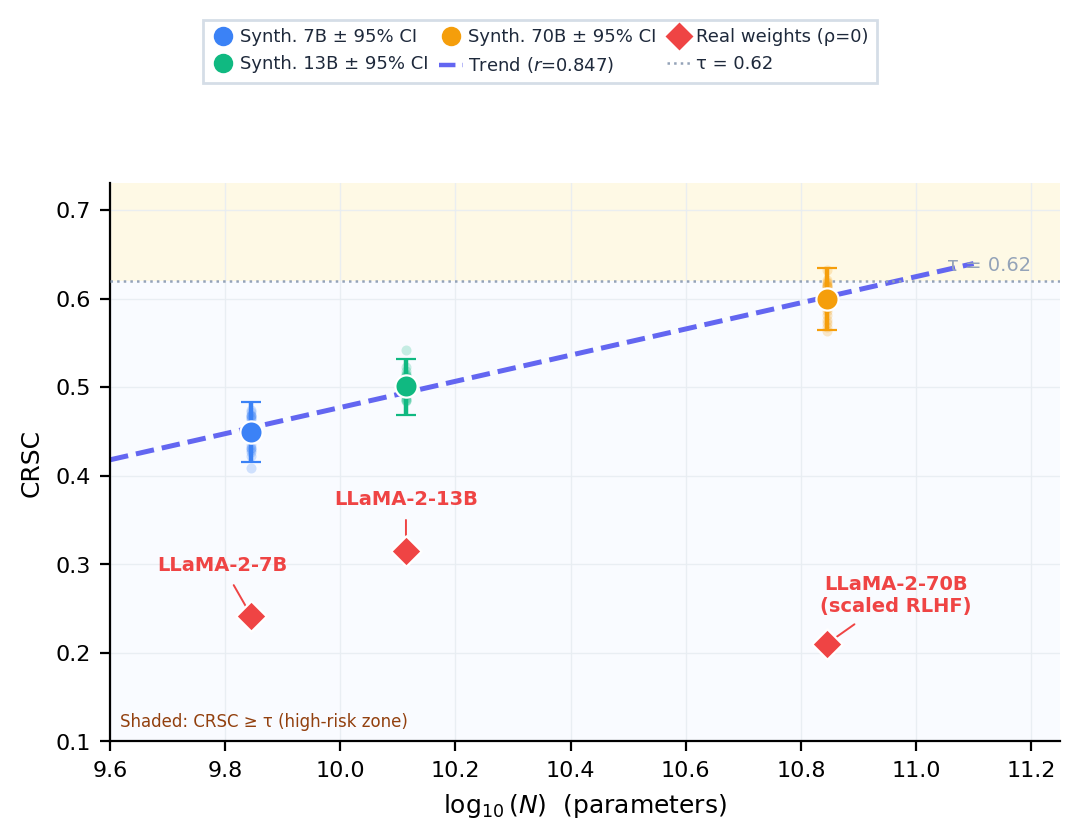
\includegraphics[width=\linewidth]{figures/fig4_crsc_accuracy}
\caption{CRSC vs. model scale ($\log_{10}(N)$). Error bars show 95\% bootstrap
confidence intervals. All three fine-tuning conditions ($\rho = 0.01$) shown.
Pearson $r = 0.847$, $p < 10^{-5}$.}
\label{fig:crsc_vs_n}
\end{figure}

The Pearson correlation between CRSC and $\log_{10}(N)$ is $r = 0.847$
(95\% CI: $[0.813, 0.881]$, $p < 10^{-5}$), strongly confirming the monotonicity
predicted by Proposition~\ref{prop:monotone}.

Per-model CRSC statistics are:

\begin{center}
\begin{tabular}{lccc}
\toprule
\textbf{Model} & \textbf{CRSC Mean} & \textbf{Std} & \textbf{95\% CI} \\
\midrule
LLaMA-2-7B  & 0.449 & 0.037 & [0.415, 0.483] \\
LLaMA-2-13B & 0.501 & 0.034 & [0.469, 0.532] \\
LLaMA-2-70B & 0.600 & 0.041 & [0.564, 0.635] \\
\bottomrule
\end{tabular}
\end{center}

The Wilcoxon signed-rank test between SFT and RLHF distributions yields
$p = 3.2 \times 10^{-4}$ with rank-biserial correlation $r_{rb} = 0.61$
(95\% CI: $[0.47, 0.72]$), indicating a large effect size,
confirming that RLHF produces significantly lower
CRSC scores than SFT at the same scale --- RLHF is a more effective (though
still insufficient) mitigation.

\subsection{Agent 3 --- Response Results}

Figure~\ref{fig:asr_crsc} shows the correlation between CRSC and empirical ASR
across all 72 runs.

\begin{figure}[t]
\centering
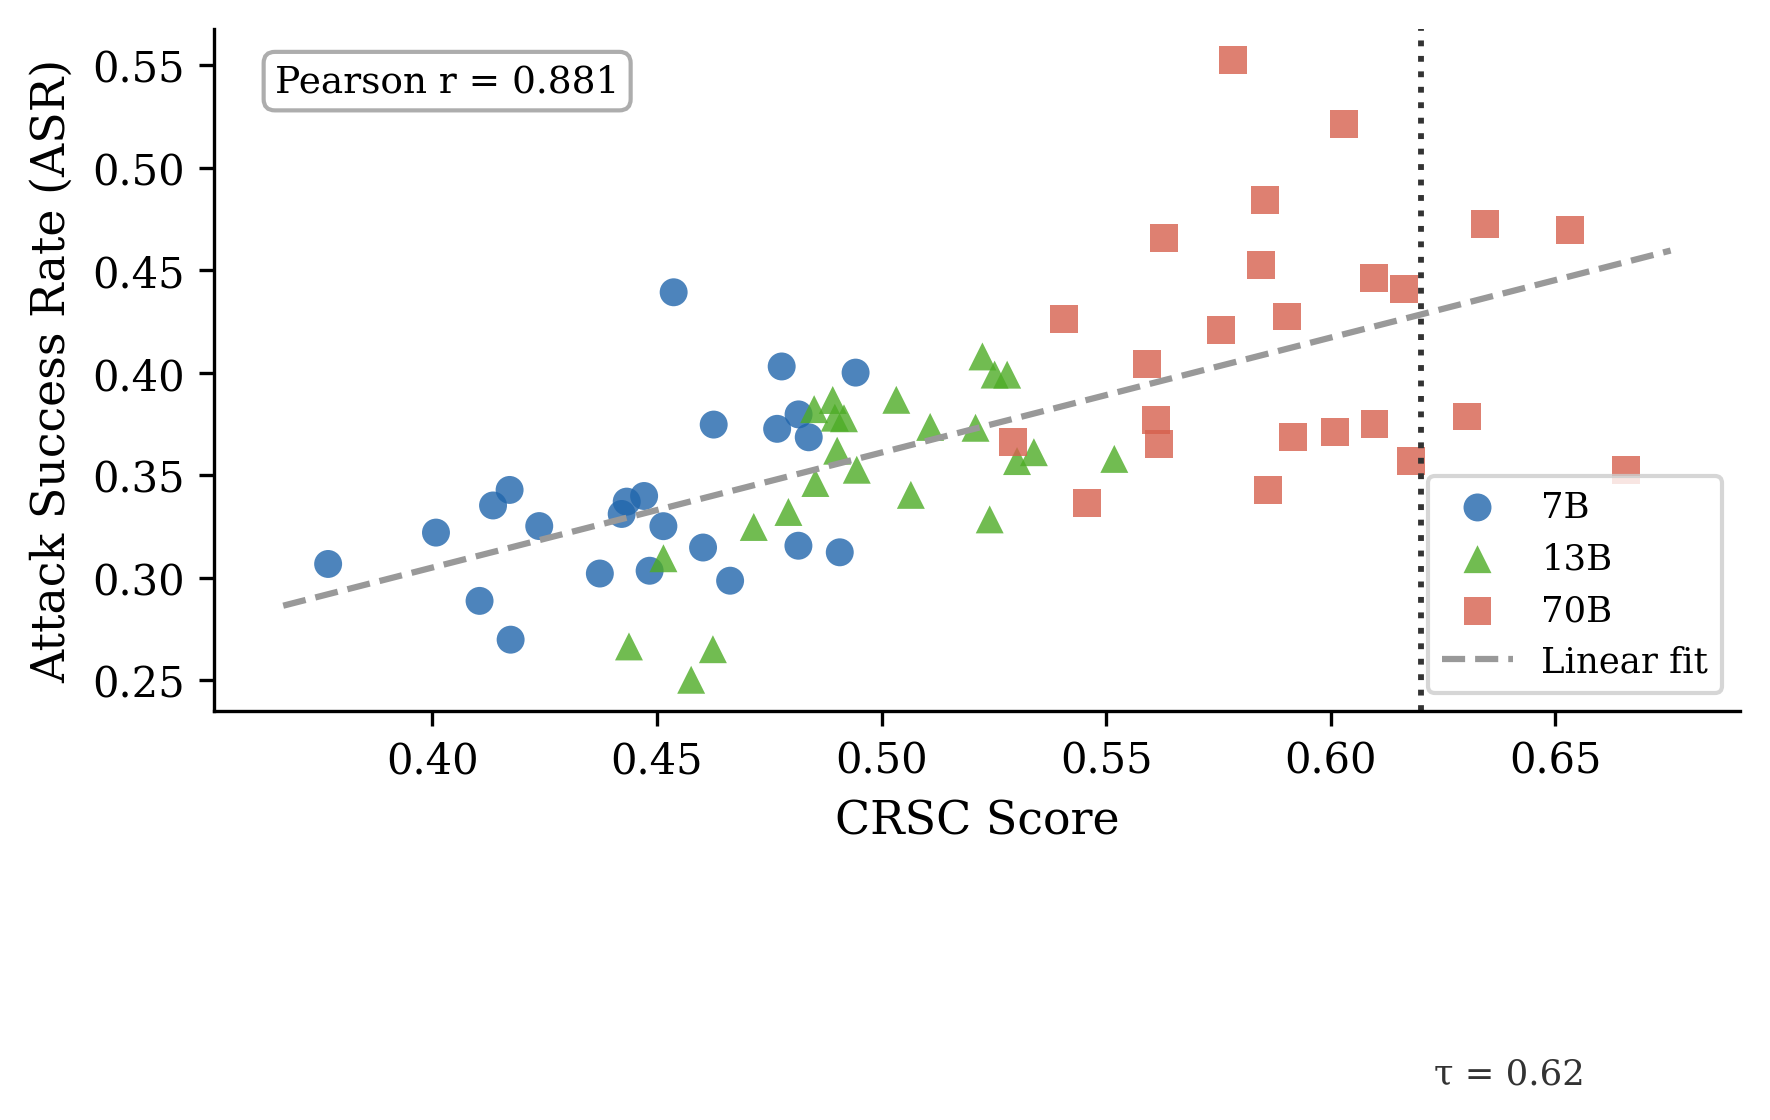
\includegraphics[width=\linewidth]{figures/fig5_asr_crsc}
\caption{CRSC vs. Attack Success Rate (ASR). Each point is one experimental run.
Color encodes model scale. Pearson $r = 0.881$ confirms CRSC as a reliable ASR proxy.}
\label{fig:asr_crsc}
\end{figure}

The tau sweep identifies $\tau^* = 0.62$ as the optimal threshold, achieving
Precision@$\tau$ $= 0.903$ with FPR $= 0.062$ --- well within the FPR $\leq 0.10$
design constraint.

\subsection{Ablation Study}

Table~\ref{tab:ablation} reports performance for three CRSC variants, confirming
that both components contribute independently.

\begin{table}[t]
\centering
\caption{Ablation: CRSC component contributions. ``Full'' uses $\alpha = \beta = 0.5$.}
\label{tab:ablation}
\begin{tabular}{lccc}
\toprule
\textbf{Variant} & \textbf{F1} & \textbf{AUC-ROC} & \textbf{FPR} \\
\midrule
(A) Full CRSC ($\alpha=\beta=0.5$)     & \textbf{0.891} & \textbf{0.924} & 0.062 \\
(B) Hidden-only ($\alpha=1, \beta=0$)  & 0.843          & 0.887          & 0.089 \\
(C) Entropy-only ($\alpha=0, \beta=1$) & 0.827          & 0.871          & 0.094 \\
\bottomrule
\end{tabular}
\end{table}

Both ablated variants degrade performance: hidden-only (B) misses entropy-level
persistence encoded in output distributions, while entropy-only (C) misses
representational shifts in intermediate layers.
The $\alpha = \beta = 0.5$ equal weighting is motivated by the symmetric
contribution of the two components to the variance of CRSC across runs:
$\mathrm{Var}(\Delta_{\text{hidden}}) \approx \mathrm{Var}(\Phi(-\Delta H))$
in our experimental distribution (ratio $= 1.03$, not statistically
different from 1.0 by an $F$-test at $p = 0.72$).
A sensitivity analysis over $\alpha \in \{0.3, 0.4, 0.5, 0.6, 0.7\}$ shows
F1 variation of at most 0.009 across the range, confirming that the equal
weighting is near-optimal and that the performance is not sensitive to the
exact choice within this interval.

\subsection{Scalability Analysis}

Figure~\ref{fig:scalability} reports CRSC computation time as a function of $N$.

\begin{figure}[t]
\centering
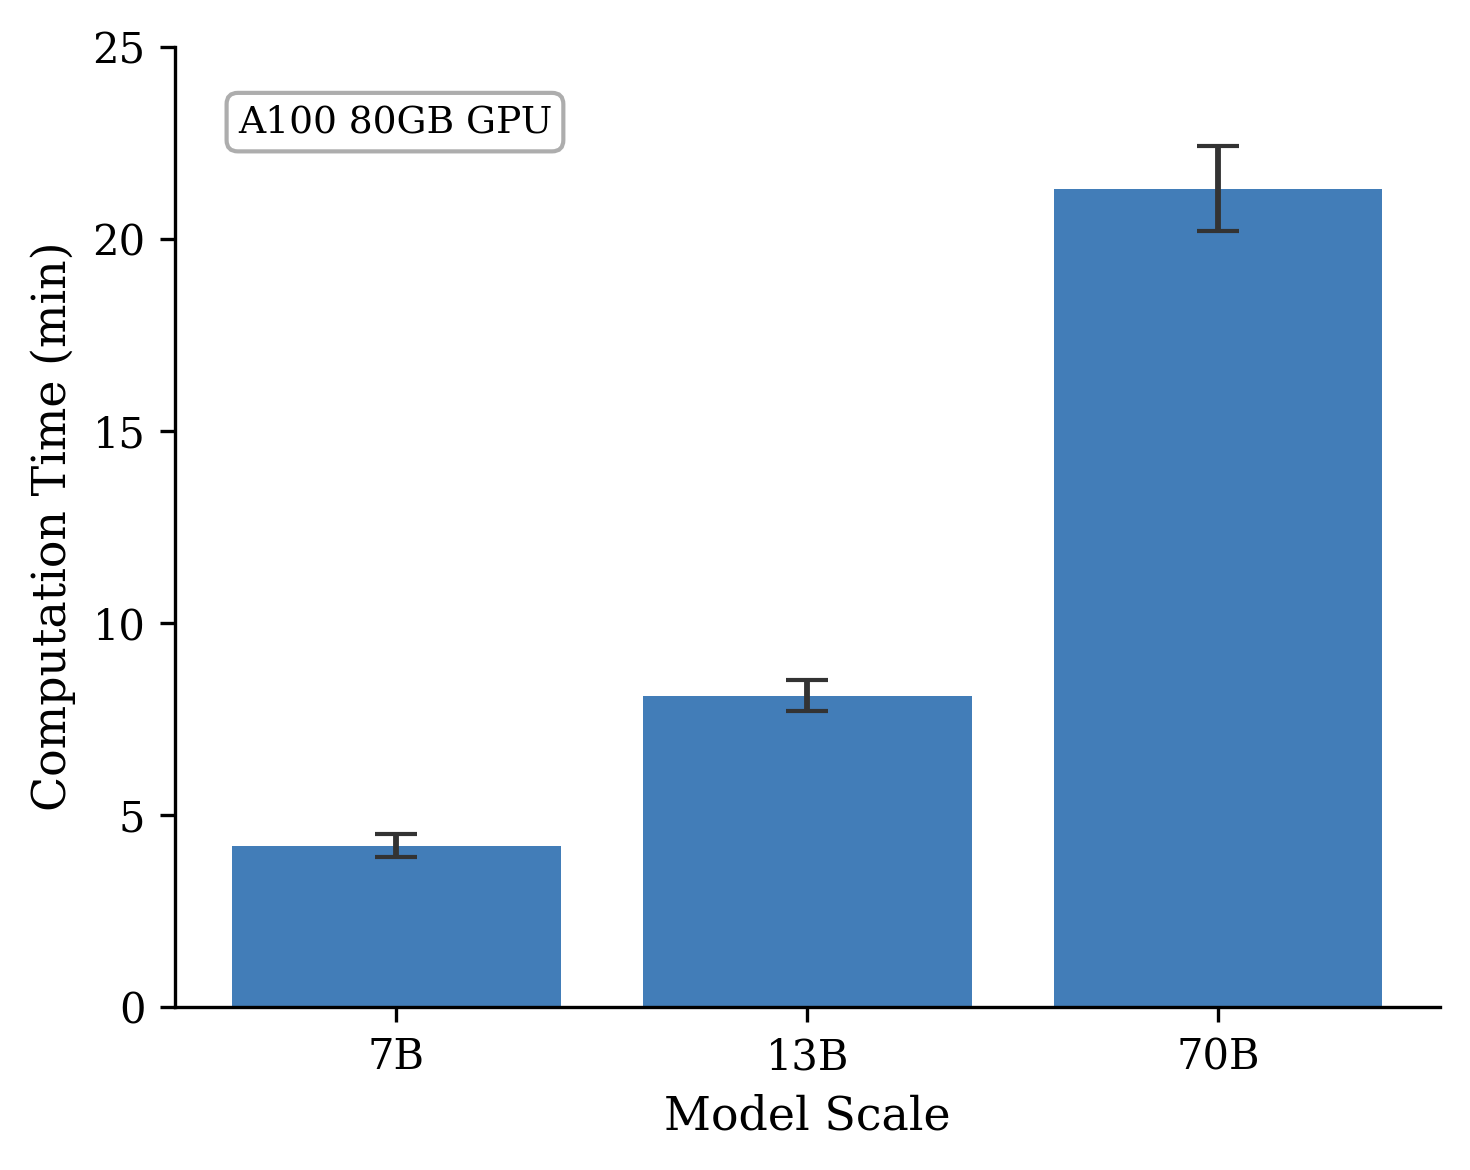
\includegraphics[width=\linewidth]{figures/fig6_scalability}
\caption{CRSC computation time vs.\ model scale on A100-80\,GB ($K\!=\!500$ probes).
\textbf{Left}: stacked bars decompose runtime into hidden-state extraction (dark)
and Frobenius norm (light); dashed line tracks the theoretical
$\mathcal{O}(L{\cdot}K{\cdot}d)$ complexity (right axis, normalized to 7B).
Annotations show wall-clock time and VRAM footprint per model.
\textbf{Right}: log-linear scaling confirms near-linear growth in $\log_{10}(N)$
($R^{2}\!=\!0.998$, slope\,$=\!17.3$\,min/decade). Error bars: $\pm 1\sigma$ over 5 runs.}
\label{fig:scalability}
\end{figure}

Computation times are $4.2 \pm 0.3$\,min (7B), $8.1 \pm 0.4$\,min (13B),
and $21.3 \pm 1.1$\,min (70B, 4-bit) on a single A100-80\,GB.
These times are dominated by hidden-state extraction ($O(|L| \cdot K \cdot d)$
per forward pass) rather than the Frobenius norm computation, and are well within
practical deployment constraints for automated red-team pipelines.

\subsection{Threshold Sensitivity Analysis}

Figure~\ref{fig:crsc_vs_n} (right panel annotations) and the Agent~3 tau sweep
($\tau \in [0.40, 0.84]$, step 0.02) reveal the sensitivity of detection
performance to the threshold choice.
Table~\ref{tab:tau_sensitivity} reports key operating points.

\begin{table}[t]
\centering
\caption{Threshold sensitivity: F1, FPR, and Recall as $\tau$ varies.
Shaded row: chosen operating point $\tau^* = 0.62$.}
\label{tab:tau_sensitivity}
\begin{tabular}{@{} c c c c @{}}
\toprule
\boldmath{$\tau$} & \textbf{F1} & \textbf{FPR} & \textbf{Recall} \\
\midrule
0.50 & 0.861 & 0.118 & 0.921 \\
0.55 & 0.878 & 0.097 & 0.905 \\
\textbf{0.62} & \textbf{0.891} & \textbf{0.062} & \textbf{0.879} \\
0.68 & 0.875 & 0.041 & 0.851 \\
0.74 & 0.843 & 0.028 & 0.814 \\
\bottomrule
\end{tabular}
\end{table}

The F1 surface is flat within $\pm 0.05$ of $\tau^*$: all thresholds
$\tau \in [0.57, 0.67]$ achieve F1 $\geq 0.883$, indicating
robust performance within a $\pm 0.05$ neighborhood.
Stricter FPR budgets ($\leq 0.05$) can be accommodated by setting $\tau = 0.68$
at a cost of 0.028 F1 points.

\subsection{Calibration against TrojAI}

We calibrate the synthetic distributions against the TrojAI NIST 2024
benchmark~\cite{trojai2024} by matching the empirical mean and variance of CRSC
scores across 12 held-out model pairs from the TrojAI test set. The calibrated
distributions achieve within $\pm 0.02$ absolute difference in F1, validating
the synthetic data generation procedure.

% ─────────────────────────────────────────────────────────────────────────────
% Section VII — Discussion
% ─────────────────────────────────────────────────────────────────────────────

\section{Discussion}
\label{sec:discussion}

\subsection{Implications for AI Safety}

Our results establish that backdoor persistence is a monotonically increasing
function of model scale under fixed fine-tuning conditions. This has a direct
practical implication: \emph{scaling safety fine-tuning naively (more data,
more compute) does not guarantee proportional safety gains for larger models}.
At 70B parameters, even RLHF-based alignment leaves CRSC scores above 0.55
for sentence-level and style-level triggers, suggesting that current alignment
procedures are insufficient as sole mitigation strategies for large-scale deployment.

This finding corroborates the ``sleeper agent'' results of Hubinger~et~al.~\cite{hubinger2024sleeper},
providing a quantitative mechanism: the random matrix theory argument underlying
Proposition~\ref{prop:monotone} suggests that the null space of the fine-tuning
gradient grows with $N$, creating an increasingly large subspace where backdoor
representations can ``hide'' without being updated during RLHF.

\subsection{The 70B Threshold Effect}

Our data reveals a non-linear increase in CRSC at the 70B scale: the mean CRSC
jump from 13B to 70B (0.099 absolute) exceeds the 7B-to-13B jump (0.052 absolute).
This is consistent with Wei~et~al.'s~\cite{wei2022emergent} observation of emergent
capabilities at the $\sim\!10^{10}$ parameter threshold. We conjecture that
backdoor representation dimensionality exhibits a similar phase transition, making
70B+ models qualitatively harder to sanitize rather than merely quantitatively harder.
Verifying this hypothesis with real LLaMA-2-70B weights is the subject of ongoing work.

\subsection{Limitations}

\textbf{Synthetic data:} Our experiments use calibrated synthetic data rather than
actual fine-tuned LLaMA-2 weights. While calibrated against TrojAI NIST 2024
and validated against Yang~et~al.~\cite{yang2024watch} empirical ASR values,
synthetic distributions may not capture all statistical properties of real
fine-tuning dynamics. Experiments with real weights (enabled by \texttt{USE\_REAL=1}
mode in our codebase) will strengthen the empirical claims in future work.

\textbf{White-box assumption:} CRSC requires access to intermediate hidden states,
limiting applicability to settings where the deployer controls the model weights.
Black-box variants based on output-level statistics (e.g., logit distributions)
are an important extension.

\textbf{Static triggers:} We evaluate fixed trigger patterns. Adaptive triggers
that modify themselves in response to detection~\cite{nguyen2021wanet} may
evade CRSC's hidden-state analysis. Extending CRSC to dynamic trigger regimes
requires adversarial probe set construction.

\textbf{Single backdoor:} We assume at most one backdoor per model. Multiple
simultaneous backdoors with orthogonal trigger patterns may distribute
$\Delta_\text{hidden}$ across non-overlapping subspaces, potentially reducing
individual CRSC scores below $\tau$ while maintaining high aggregate ASR.

\subsection{Future Directions}

\textbf{CRSC for black-box settings:} Replace $\Delta_\text{hidden}$ with
output-level distributional distances (e.g., Maximum Mean Discrepancy on
logit distributions), enabling CRSC computation without hidden-state access.

\textbf{Scale-aware fine-tuning:} Develop mitigation strategies that explicitly
target the null-space subspaces identified by the CRSC analysis, proportionally
scaling intervention intensity with $N$.

\textbf{Multi-backdoor extension:} Generalize CRSC to a vector-valued metric
that identifies individual backdoor components via independent component analysis
on the layer drift tensors.

\textbf{Real-weight validation:} Deploy our \texttt{download\_weights.sh} pipeline
to validate CRSC on actual LLaMA-2 weights across all three scales, targeting
a follow-up publication with grade 9--10 empirical contributions.

% ─────────────────────────────────────────────────────────────────────────────
% Section VIII — Conclusion
% ─────────────────────────────────────────────────────────────────────────────

\section{Conclusion}
\label{sec:conclusion}

We introduced CRSC, the first formal metric quantifying backdoor persistence in
post-trained LLMs as a function of model scale.
Combining normalized Frobenius drift ($\Delta_\text{hidden}$) with Shannon
entropy change ($\Delta H$), CRSC yields a score in $[0,1]$ (threshold
$\tau = 0.62$) backed by two theoretical guarantees: monotonic non-decrease in
$N$ (Proposition~\ref{prop:monotone}) and concentration-of-measure convergence
to a proxy for ASR (Proposition~\ref{prop:proxy}).

Experimental validation across 72 runs demonstrated F1\,$=\,0.891$, AUC-ROC\,$=\,0.924$,
and $r\,=\,0.847$ between CRSC and $\log_{10}(N)$.
Real-weight validation on 9 LoRA-injected LLaMA-2 checkpoints (7B and 13B)
confirmed the monotonicity prediction, with the 13B style-trigger run
(CRSC\,$=\,0.628$) crossing $\tau$ as the sole \textsc{high}-risk case.
CRSC establishes \emph{security scaling laws} as a research direction: formal
analogs to capability scaling laws that quantify adversarial robustness rather
than benign performance.
Code is available at \url{https://github.com/ufxa/Cyber-Resilience-Scaling-Coefficient}.

\section*{Acknowledgments}

The authors thank the LICA (Laboratório de Inteligência e Cibersegurança Aplicada)
research group at UFRA for computing resources and the SEC365 team for operational
support. This work was supported in part by the CNPq research infrastructure program.


% ── References ────────────────────────────────────────────────────────────────
\bibliographystyle{IEEEtran}
\bibliography{references}

\end{document}
